\newpage
\chapter{METODE PENELITIAN} \label{Bab III}

\section{Alur Penelitian} \label{III.Alur}

Alur penelitian ini menggambarkan tahapan yang dilakukan dari awal hingga akhir untuk menyelesaikan penelitian mengenai deteksi kejatuhan manusia menggunakan \textit{Graph Convolutional Network} (GCN) berbasis \textit{pose landmark}. Alur penelitian digambarkan dalam bentuk \textit{flowchart} berikut.\par

\begin{figure}[H]  % 'h' menunjukkan gambar akan diletakkan di sekitar posisi ini
    \centering  % Gambar dipusatkan
    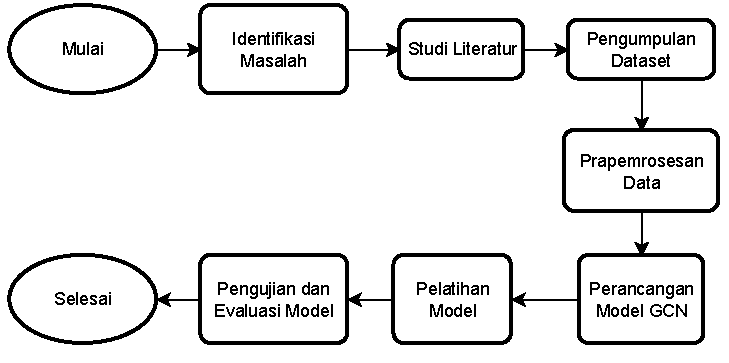
\includegraphics[width=0.9\textwidth]{figure/BAB 3/alur penelitian.pdf}  % Menyisipkan gambar dengan lebar setengah lebar teks
    \caption{Alur penelitian.}  % Menambahkan keterangan gambar
    \label{fig:alur penelitian}  % Menambahkan label untuk referensi
\end{figure}

Tahapan-tahapan yang dilakukan dalam penelitian secara keseluruhan terlihat pada gambar \ref{fig:alur penelitian}. Proses dimulai dengan identifikasi masalah dan tujuan penelitian untuk menentukan fokus dan arah dari penelitian. Selanjutnya, dilakukan Studi Literatur untuk memahami penelitian sebelumnya yang relevan agar menambah wawasan dan menemukan kekurangan atau area yang dapat ditingkatkan dalam bidang tersebut. Setelah itu, dilakukan Pengumpulan dataset yang mencakup pengumpulan dataset video yang dibutuhkan untuk eksperimen. \par

Tahapan berikutnya adalah prapemrosesan data dan ekstraksi fitur, di mana data yang terkumpul diolah dan dipersiapkan untuk digunakan dalam model. Ini mencakup ekstraksi \textit{frame} dan pengolahan data \textit{pose landmark}. Kemudian Membangun model GCN dilakukan untuk merancang dan menyusun model yang akan digunakan dalam penelitian ini. Selanjutnya, dilakukan pelatihan model menggunakan dataset yang telah diproses, diikuti dengan evaluasi performa model untuk mengukur akurasi dan kinerja model dalam mendeteksi posisi jatuh pada lansia. Proses ini berulang, dengan model terus diperbaiki berdasarkan hasil evaluasi. Akhirnya, setelah seluruh tahapan selesai. \par

\section{Penjabaran Alur Penelitian} \label{III.Jabar Alur}
Subbab ini akan menjelaskan setiap langkah dalam alur penelitian secara detail dan menyeluruh. Subbab ini bertujuan untuk memperjelas alur penelitian dan mencegah munculnya berbagai pemikiran atau pendapat yang keliru mengenai penelitian ini. Seluruh langkah penelitian yang telah ditampilkan pada subbab \ref{III.Alur} akan dijabarkan secara rinci sebagai berikut. \par

\subsection{Identifikasi Masalah} \label{III.identifikasi masalah}
Tahap pertama dari penelitian ini adalah memulai proses yang mencakup pemahaman mendalam tentang tujuan dari penelitian ini serta pengaturan langkah-langkah yang akan diambil. Penelitian ini dimulai dengan menetapkan gambaran besar dan objektif penelitian, dengan masalah utama yang dihadapi adalah tingginya angka kecelakaan yang terjadi pada lansia, terutama yang disebabkan oleh kejadian jatuh yang kurang diperhatikan. Jatuh pada lansia sering kali mengakibatkan cedera serius dan bahkan kematian. \par

Berdasarkan permasalahan jatuh tersebut, penelitian ini berfokus untuk mengembangkan model deteksi posisi jatuh yang dapat membantu mengidentifikasi kejadian jatuh dengan cepat, yang berpotensi menyelamatkan nyawa. Berdasarkan seluruh informasi tersebut, maka tujuan dari penelitian ini adalah  merancang dan membangun model yang dapat menganalisis data \textit{pose landmark} tubuh dari lansia menggunakan Mediapie, lalu memanfaatkan teknologi GCN untuk mendeteksi posisi jatuh berdasarkan data tersebut. \par

\subsection{Studi Literatur} \label{III.studi literatur}
Langkah ini dapat dikatakan sebagai pondasi utama dalam penelitian ini. Lankah-langkah selanjut nya dalam alur penelitian ini tentunya membutuhkan pengetahuan mendalam yang bisa didapatkan dari berbagai sumber, salah satunya literatur penelitian. Berbagai literatur terdahulu yang berkaitan dengan penelitian ini harus dipelajari, dengan kalimat kunci antara lain \textit{Graph Convolutional Network} (GCN), Kejadian jatuh pada lansia, Mediapipe, \textit{pose Landmark}, dan sebagainya. \par

\subsection{Pengumpulan Dataset} \label{III.pengumpulan data}
Langkah selanjutnya adalah pengumpulan dataset yang diperlukan untuk penelitian. Ditemukan dataset\footnote{https://iiw.kuleuven.be/onderzoek/advise/datasets\#High\%20Quality\%20Fall\%20Simulation\%20Data} yang telah disediakan dalam Paper "\textit{Bridging the gap between real-life data and simulated data by providing realistic fall dataset for evaluating camera-based fall detection algorithms}". Dataset ini berupa video gerakan tubuh yang diambil menggunakan kamera 2 dimensi. Pembuatan dataset ini bertujuan untuk mendokumentasikan berbagai skenario dalam lingkungan yang realistis. Skenario jatuh yang berbeda dirancang untuk meniru insiden jatuh yang sebenarnya dengan seakurat mungkin. \par

\begin{figure}[htbp]  % 'h' menunjukkan gambar akan diletakkan di sekitar posisi ini
    \centering  % Gambar dipusatkan
    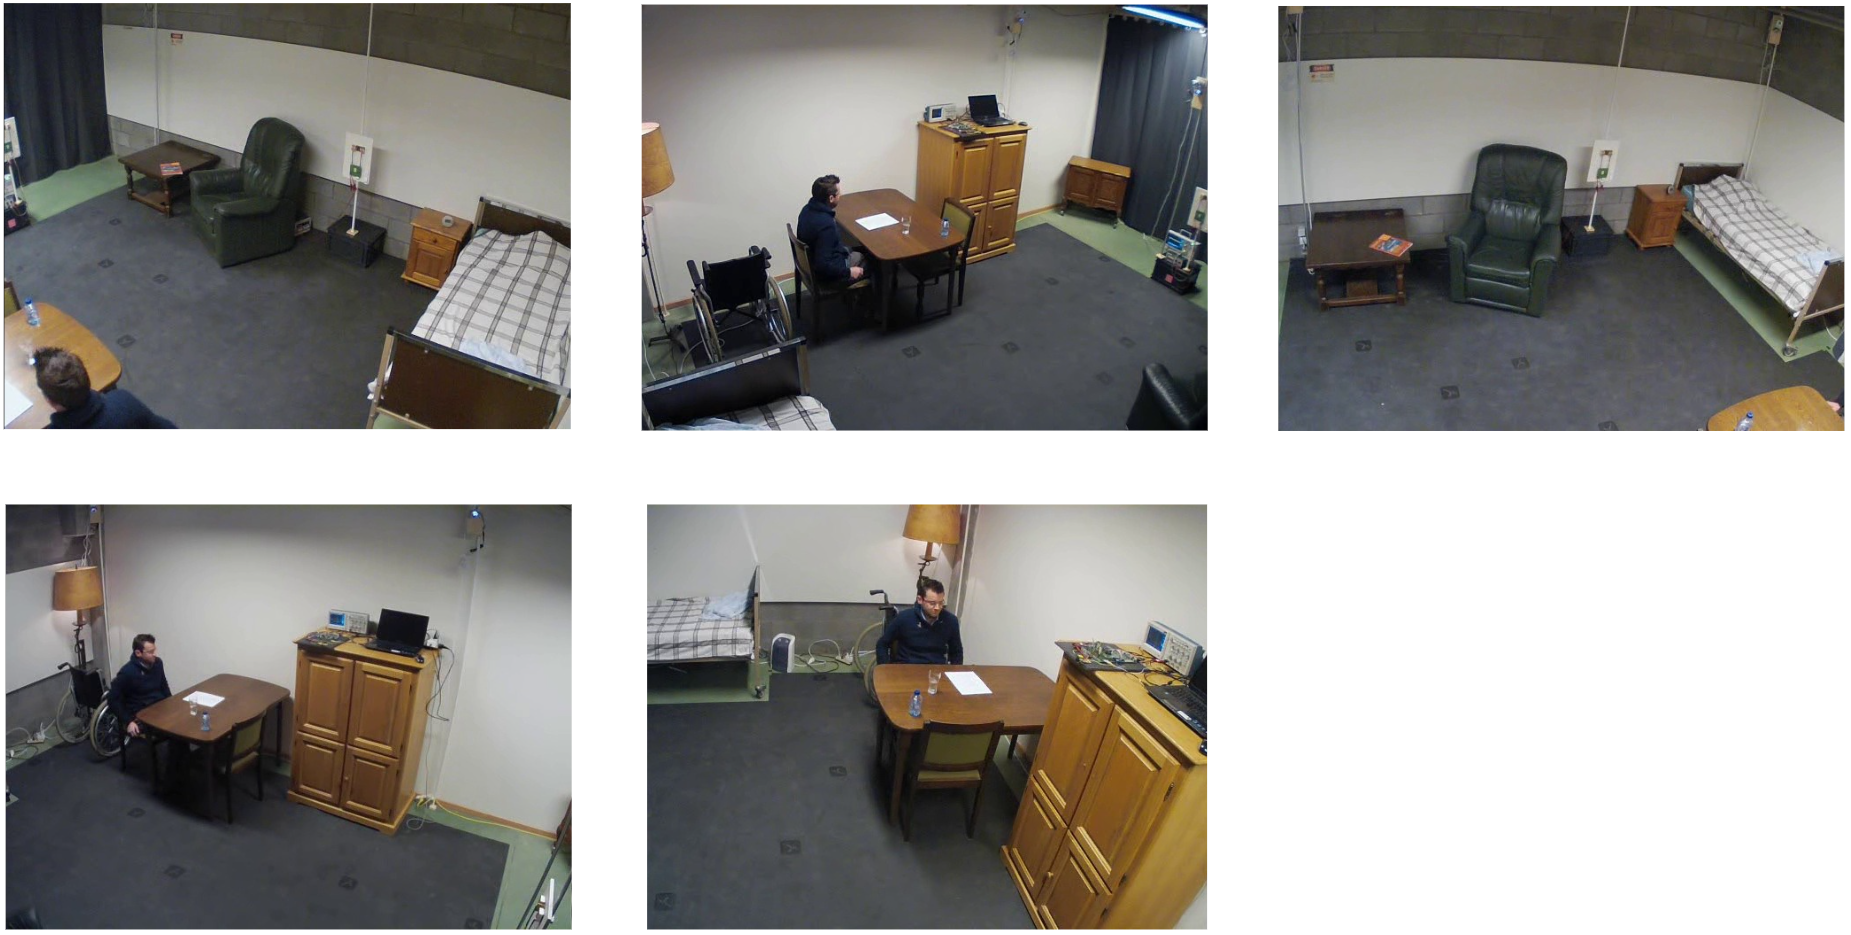
\includegraphics[width=0.9\textwidth]{figure/BAB 3/Preview 5 sudut kamera dataset.png}  % Menyisipkan gambar dengan lebar setengah lebar teks
    \caption{\textit{Preview} dataset dengan 5 sudut pandang kamera}  % Menambahkan keterangan gambar
    \label{fig:preview 5 sudut kamera}  % Menambahkan label untuk referensi
\end{figure}

Dataset tersebut terdiri dari 54 skenario jatuh dan 17 skenario tidak jatuh. Masing-masing skenario direkam dengan 5 sudut pandang seperti yang terlihat pada Gambar \ref{fig:preview 5 sudut kamera}, sehingga menghasilkan 270 video jatuh dan 85 video tidak jatuh. Video skenario jauh memiliki rentang durasi 1 - 5 menit, sedangkan skenario tidak jatuh berkisar 10 - 30 menit. Seluruh video tersebut memiliki ukuran fram 800 x 480 piksel. Disediakan juga file meta yang berisi informasi rinci dari setiap video, misalnya setiap video jatuh disediakan informasi aktor, kondisi mulai jatuh, kondisi akhir jatuh dan deskripsi skenario. Terdapat juga penanda waktu mulai jatuh, tepat jatuh, berakhirnya jatuh dan durasi kejadian jatuh dalam satuan detik. Sama halnya dengan video tidak jatuh disediakan deskripsi skenario, durasi video dan aktor.\par

\subsection{Prapemrosesan Data} 
\label{III.prapemrosesan}

\begin{figure}[htbp]  % 'h' menunjukkan gambar akan diletakkan di sekitar posisi ini
    \centering  % Gambar dipusatkan
    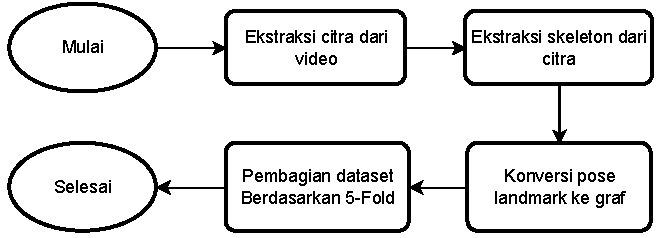
\includegraphics[width=1\textwidth]{figure/BAB 3/alur_prapemrosesan_dataset.pdf}  % Menyisipkan gambar dengan lebar setengah lebar teks
    \caption{Alur prapemrosesan dataset}  % Menambahkan keterangan gambar
    \label{fig: alur prapemrosesan}  % Menambahkan label untuk referensi
\end{figure}

Pada subbab ini akan dijelaskan secara rinci alur prapemrosesan dataset agar dapat diterima oleh model untuk melakukan pelatihan. Terlihat pada Gambar \ref{fig: alur prapemrosesan}, secara garis besar terdapat 4 tahap yaitu mengekstraksi citra yang diperlukan dari setiap video yang ada dalam dataset, lalu mengunakan \textit{Mediapipe Pose} untuk mendeteksi 33 \textit{pose landmark} manusia dari tiap citra yang disertai dengan penyesuaian jumlah data pada masing-masing kelas jika total data tidak setara, kemudian melakukan konversi data \textit{pose landmark} tersebut ke dalam bentuk graf, dan terakhir melakukan pembagian data dengan menerapkan 5-Fold agar menghindari kebocoran data saat pelatihan model. Seluruh tahapan harus dilakukan agar model GCN dapat memproses dan mempelajari pola dan hubungan spasial tiap \textit{landmark} sehingga dapat memprediksi posisi jatuh dan tidak jatuh pada manusia secara akurat. \par

\subsubsection{Ekstraksi Citra Dari Video}
\label{III.ekstrak citra}
Prapemrosesan awal terhadap dataset dilakukan dengan mengekstrak 30 citra dari rentang detik di setiap video dalam dataset. Langkah ini bertujuan untuk mengurangi ukuran data yang akan diproses dan memastikan bahwa analisis dilakukan hanya pada \textit{frame} citra yang relevan, baik kejadian jatuh maupun tidak jatuh. Mencapai tujuan tersebut, program Python ekstraksi \textit{frame} perlu dikembangkan agar dapat secara otomatis mengekstrak citra berdasarkan informasi penanda waktu yang disediakan dalam file meta. \par

File meta ini berisi data penanda waktu yang menandakan waktu mulai dan berakhirnya kejadian yang khusus untuk video jatuh, namun sayangnya tidak disediakan penanda waktu untuk video tidak jatuh sehingga harus ditentukan secara manual penanda waktu mulai dan berakhir suatu kejadian dalam video tidak jatuh tersebut. Data ini dapat digunakan untuk menentukan waktu yang tepat untuk ekstraksi citra. Program Python ini akan membaca file meta untuk memperoleh informasi penanda waktu jatuh dan kemudian memilih 30 \textit{frame} citra secara acak di sepanjang periode tersebut. \par

% \begin{figure}[htbp]  % 'h' menunjukkan gambar akan diletakkan di sekitar posisi ini
%     \centering  % Gambar dipusatkan
%     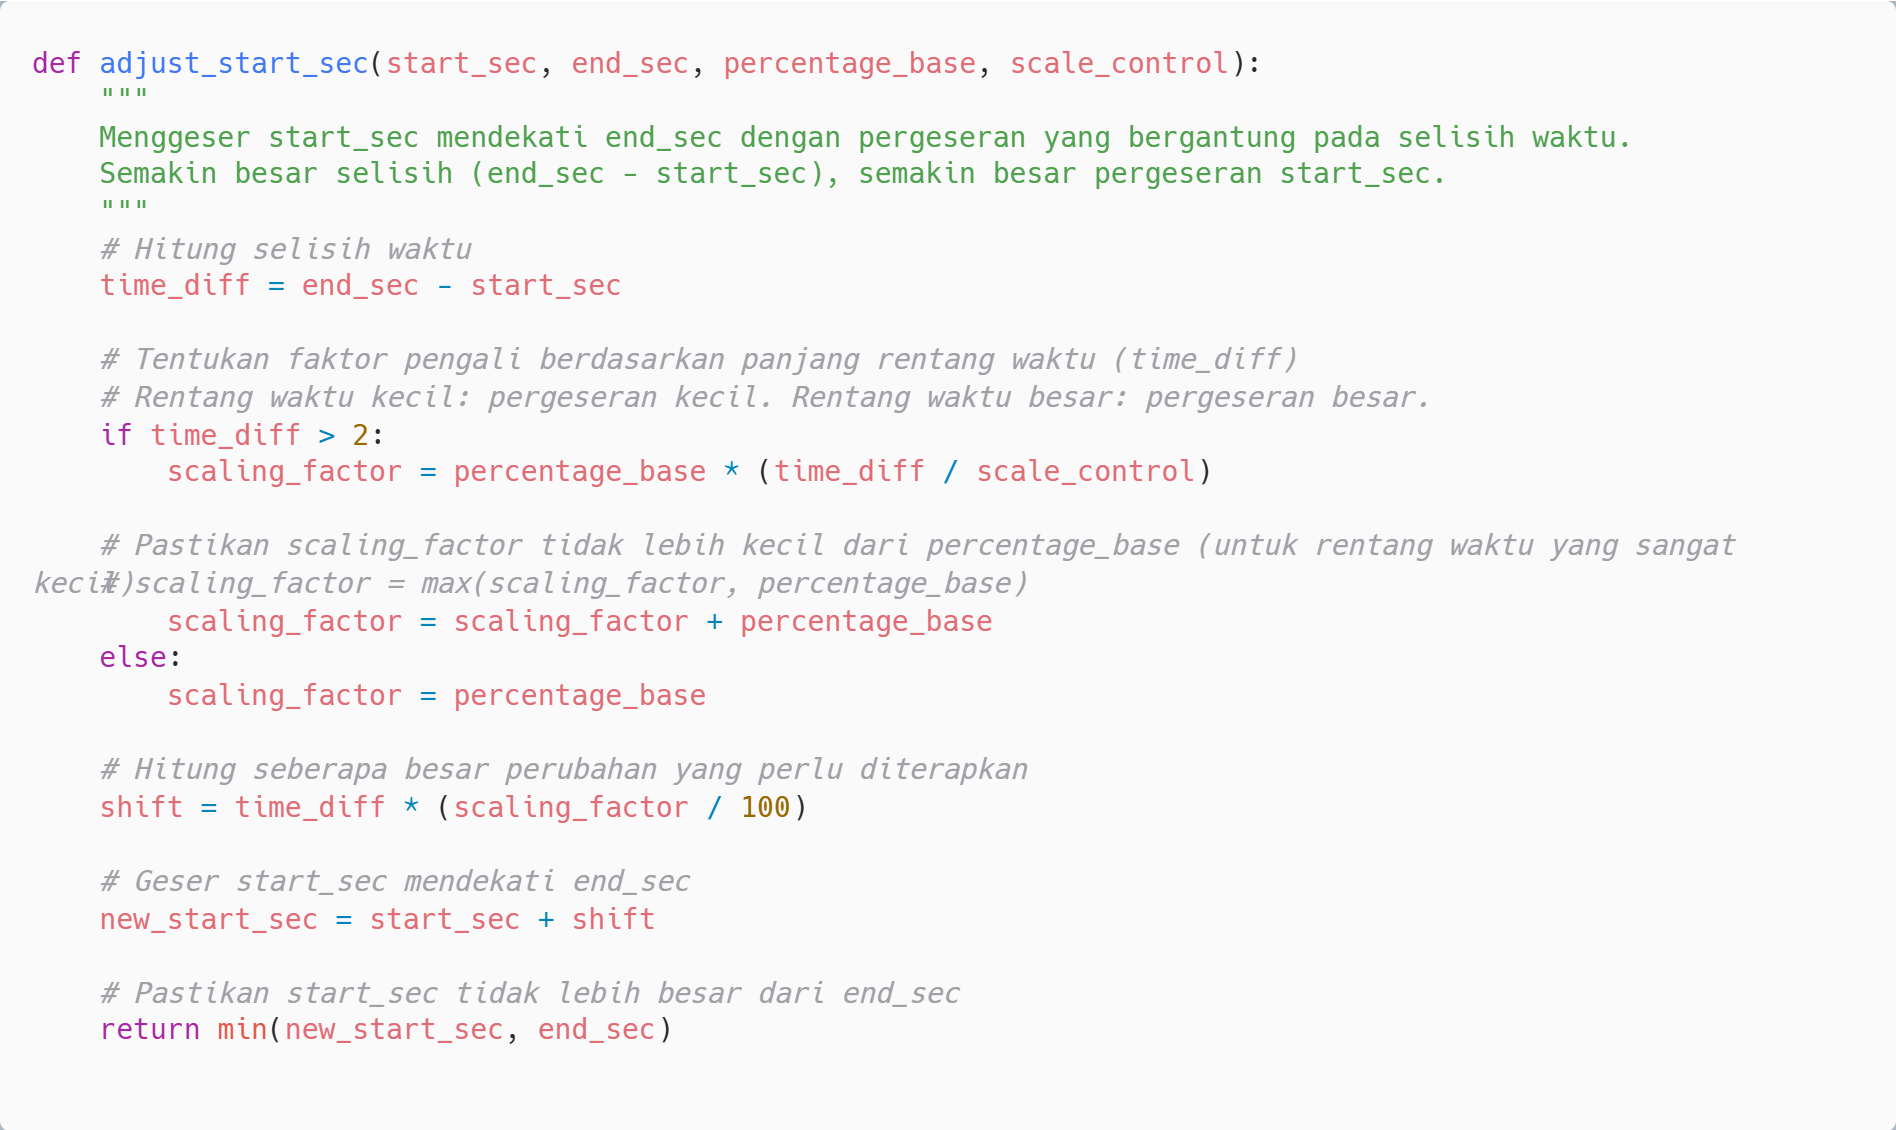
\includegraphics[width=1\textwidth]{images/adjust_start-sec.png}  % Menyisipkan gambar dengan lebar setengah lebar teks
%     \caption{Kode pergeseran \textit{start\_time}}  % Menambahkan keterangan gambar
%     \label{fig:kode pergeseran waktu mulai}  % Menambahkan label untuk referensi
% \end{figure}

\begin{lstlisting}[language=Python, caption={Pergeseran \textit{start\_time}}, label={kode:pergeseran waktu mulai}]
def adjust_start_sec(start_sec, end_sec, percentage_base, scale_control):
    """
    Menggeser start_sec mendekati end_sec dengan pergeseran yang bergantung pada selisih waktu.
    Semakin besar selisih (end_sec - start_sec), semakin besar pergeseran start_sec.
    """
    # Hitung selisih waktu
    time_diff = end_sec - start_sec
    
    # Tentukan faktor pengali berdasarkan panjang rentang waktu (time_diff)
    # Rentang waktu kecil: pergeseran kecil. Rentang waktu besar: pergeseran besar.
    if time_diff > 2:
        scaling_factor = percentage_base * (time_diff / scale_control)
    
    # Pastikan scaling_factor tidak lebih kecil dari percentage_base (untuk rentang waktu yang sangat kecil)
    # scaling_factor = max(scaling_factor, percentage_base)
        scaling_factor = scaling_factor + percentage_base
    else:
        scaling_factor = percentage_base
    
    # Hitung seberapa besar perubahan yang perlu diterapkan
    shift = time_diff * (scaling_factor / 100)
    
    # Geser start_sec mendekati end_sec
    new_start_sec = start_sec + shift
    
    # Pastikan start_sec tidak lebih besar dari end_sec
    return min(new_start_sec, end_sec)
\end{lstlisting}

\vspace{10pt}

% \begin{lstlisting}[caption={Kode ekstrak frame acak}, label={kode:ekstrak random}]


% \end{lstlisting}

Potongan Kode pada Kode \ref{kode:pergeseran waktu mulai} merupakan fungsi \textit{adjust\_start\_sec} yang dipakai khusus untuk video berlabel jatuh guna “menggeser” waktu mulai (start\_sec) mendekati waktu akhir (end\_sec) secara proporsional terhadap panjang rentang kejadian. logika utamanya yaitu bila durasi interval besar, bagian awal yang kurang relevan dikurangi lebih banyak sehingga sampling frame lebih terfokus ke momen inti menjelang jatuh. Nilai balik dibatasi agar tidak melewati \textit{end\_sec}. \par

% \begin{figure}[htbp]  % 'h' menunjukkan gambar akan diletakkan di sekitar posisi ini
%     \centering  % Gambar dipusatkan
%     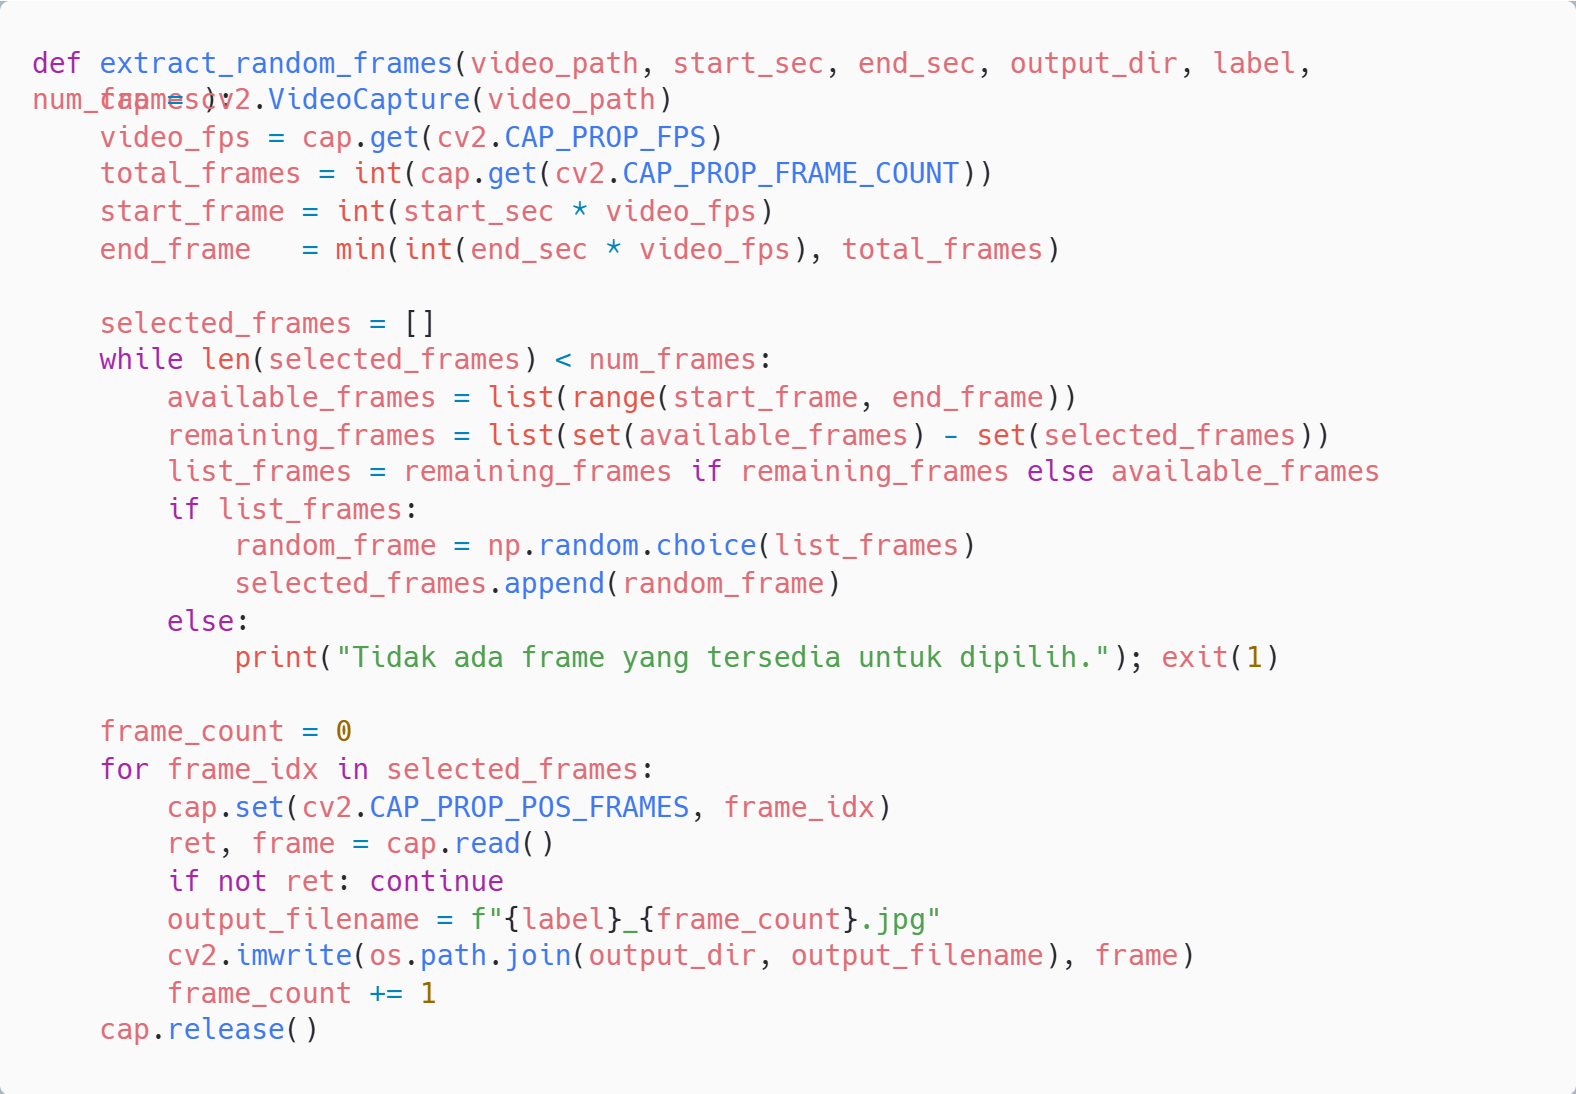
\includegraphics[width=1\textwidth]{images/extract_random_frames.png}  % Menyisipkan gambar dengan lebar setengah lebar teks
%     \caption{Kode ekstrak frame acak}  % Menambahkan keterangan gambar
%     \label{fig:kode ekstrak random}  % Menambahkan label untuk referensi
% \end{figure}


\begin{lstlisting}[caption={Ekstrak frame acak}, label={kode:ekstrak random}]
def extract_random_frames(video_path, start_sec, end_sec, output_dir, label, num_frames=30):
    """
    Mengekstrak frame secara acak dalam rentang waktu yang telah disesuaikan.
    Jika frame unik kurang dari 30, ambil frame yang sama secara acak hingga mencapai jumlah 30 frame.
    """
    
    if os.path.exists(output_dir):
        return
    
    os.makedirs(output_dir, exist_ok=True)
    
    cap = cv2.VideoCapture(video_path)
    video_fps = cap.get(cv2.CAP_PROP_FPS)
    total_frames = int(cap.get(cv2.CAP_PROP_FRAME_COUNT))
    
    start_frame = int(start_sec * video_fps)
    end_frame = min(int(end_sec * video_fps), total_frames)
    
    # Membuat daftar untuk frame yang dipilih
    selected_frames = []
    
    # Ambil frame secara acak hingga semua frame dalam rentang terambil
    while len(selected_frames) < num_frames:
        # Pilih frame acak dalam rentang waktu yang diberikan
        available_frames = list(range(start_frame, end_frame))
        
        # Pilih frame yang belum diambil
        remaining_frames = list(set(available_frames) - set(selected_frames))
        
        if remaining_frames:
            # Pilih frame acak dari yang tersisa
            random_frame = np.random.choice(remaining_frames)
            selected_frames.append(random_frame)
        else:
            # Jika semua frame unik sudah diambil, ambil secara acak lagi sampai mencapai 30 frame
            random_frame = np.random.choice(available_frames)
            selected_frames.append(random_frame)
    
    # Ekstraksi frame yang telah dipilih
    frame_count = 0
    for frame_idx in selected_frames:
        cap.set(cv2.CAP_PROP_POS_FRAMES, frame_idx)
        ret, frame = cap.read()
        if not ret:
            continue
        
        output_filename = f"{label}_{frame_count}.jpg"
        cv2.imwrite(os.path.join(output_dir, output_filename), frame)
        frame_count += 1
    
    cap.release()
\end{lstlisting}

\vspace{10pt}

Fungsi \textit{extract\_random\_frames} pada Kode \ref{kode:ekstrak random} adalah inti ekstraksi. Fungsi ini membuka video, menghitung indeks frame berdasarkan \textit{start\_sec\–end\_sec}, lalu memilih secara acak sejumlah \textit{num\_frames} dari rentang tersebut. Jika frame unik tidak cukup, program mengizinkan pengambilan ulang secara acak hingga kuota terpenuhi. Setiap frame terpilih disimpan sebagai citra di folder keluaran dengan penamaan yang menyertakan label kelas. \par

Secara keseluruhan, program ekstraksi citra akan dimulai dengan membuka dan membaca file meta dataset tersebut menggunakan \textit{library Pandas}. Informasi penanda waktu mulai dan berakhirnya kejadian jatuh serta tidak jatuh sebagai acuan program untuk menentukan titik awal dan akhir kejadian di setiap video. Video jatuh berjumlah 270 dan video tidak jatuh sebanyak 85. Berdasarkan penanda waktu dalam file meta, program akan memilih 30 \textit{frame} yang tersebar merata secara acak selama durasi kejadian jatuh untuk mendapatkan data yang representatif dari kejadian tersebut. Misalnya, jika durasi jatuh adalah 2 detik, maka 30 \textit{frame} akan dipilih selama rentang waktu tersebut. Sementara itu, jumlah video jatuh dan tidak jatuh berbeda, sehingga perlu melakukan penyesuaian jumlah video dengan membagi masing-masing video dengan mengambil durasi tertentu berdasarkan aksi aktor, sehingga didapatkan total video tidak jatuh sebanyak 270. \par

Program kemudian akan mengekstrak \textit{frame} sesuai dengan penanda waktu yang telah ditentukan menggunakan \textit{library OpenCV}, mengidentifikasi posisi \textit{frame} pada penanda waktu yang ditetapkan, dan menyimpan hasil ekstraksi citra dalam format yang sesuai seperti JPG. Berikut perhitungan sederhana untuk melihat jumlah frame citra yang akan didapatkan. \par

\begin{align*}
    \text{Total citra} &= (\text{total video jatuh} \times 30) +(\text{total video tidak jatuh} \times 30) \label{eq:total citra}\\
    &= (270 \times 30) + (270 \times 30) = 8.100 + 8.100 = 16.200
\end{align*}
\vspace{7pt}

berdasarkan perhitungan tersebut, diperkirakan total frame citra yang akan didapatkan sebanyak 16.200. Hasil ekstraksi \textit{frame} ini akan disimpan dalam folder yang terorganisir dengan baik berdasarkan video dan informasi terkait, sehingga memudahkan analisis lebih lanjut. Contoh \textit{frame} citra yang akan didapatkan dari video dataset dapat dilihat pada Gambar \ref{fig:contoh frame}. \par

\begin{figure}[htbp]  % 'h' menunjukkan gambar akan diletakkan di sekitar posisi ini
    \centering  % Gambar dipusatkan
    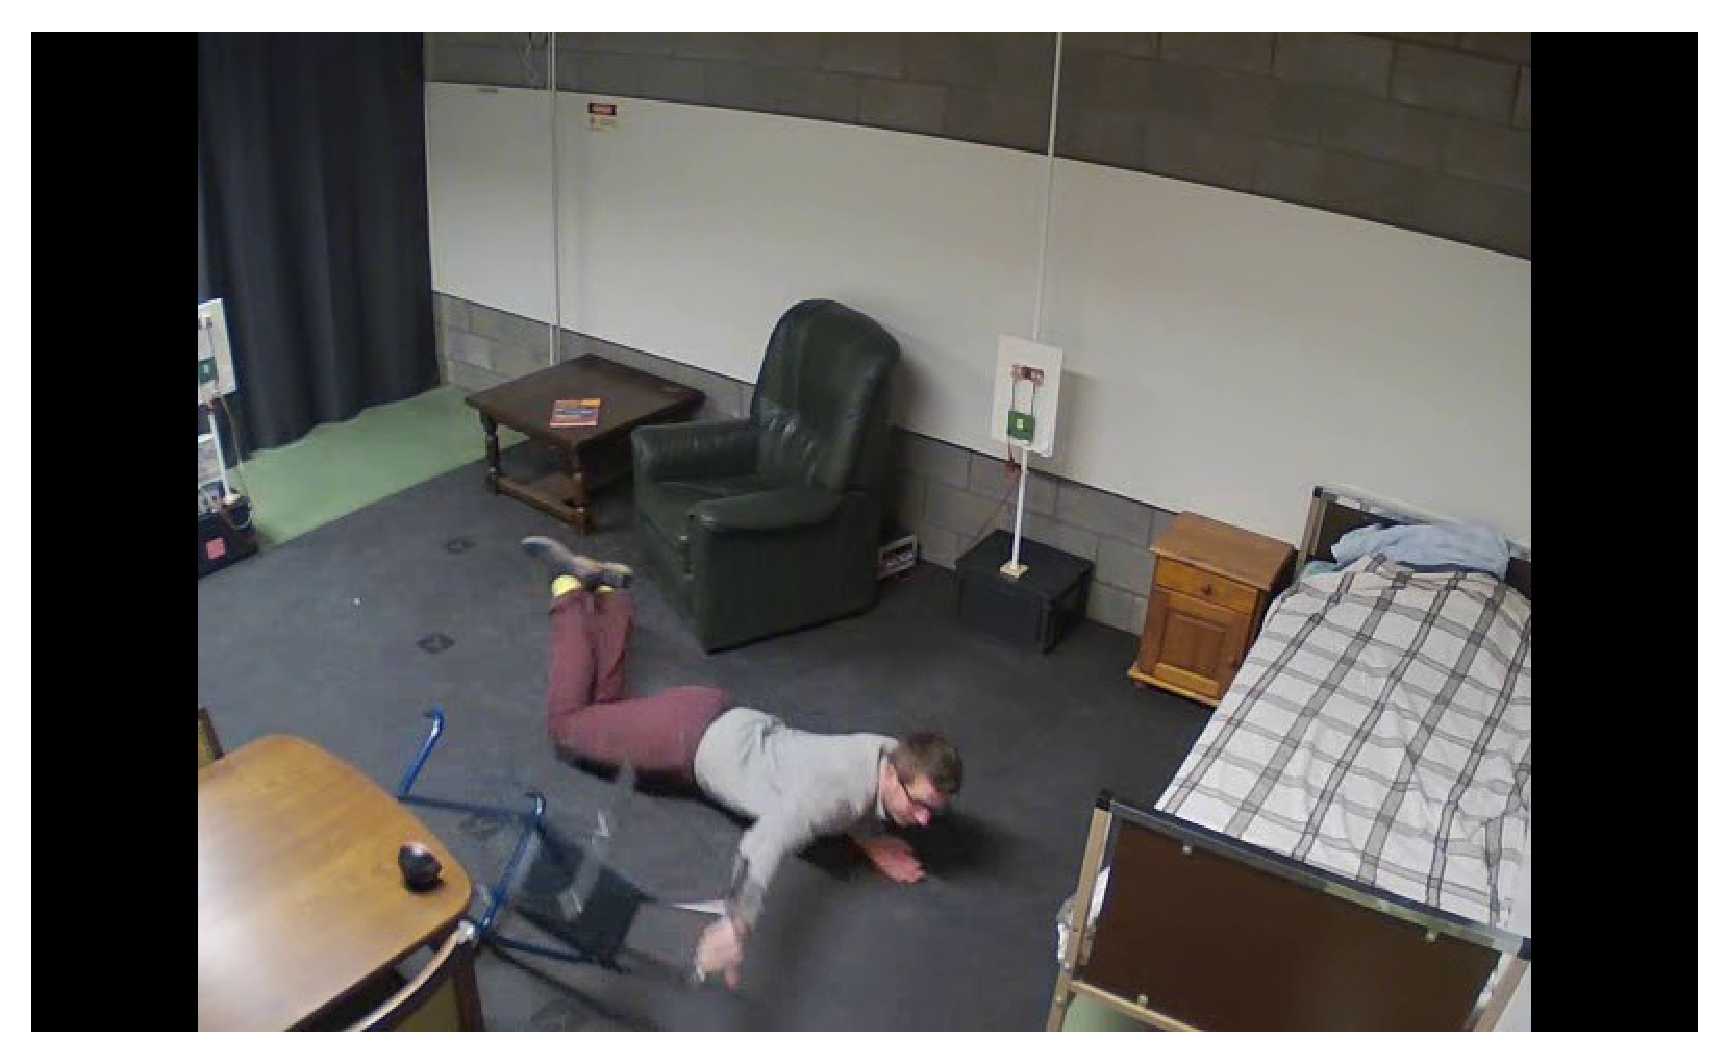
\includegraphics[width=0.7\textwidth, trim=3.5cm 0 3.5cm 0, clip]{figure/BAB 3/contoh citra jatuh.pdf}  % Menyisipkan gambar dengan lebar setengah lebar teks
    \caption{contoh citra dari video jatuh.}  % Menambahkan keterangan gambar
    \label{fig:contoh frame}  % Menambahkan label untuk referensi
\end{figure}

\subsubsection{Deteksi 33 \textit{Landmark} Dengan\textit{ Mediapipe Pose}}
\label{III.deteksi pose landmark}
% tambahin sitasi 
Proses selanjutnnya yaitu seluruh citra tersebut akan diproses menggunakan \textit{framework mediapipe} untuk mendapatkan data \textit{pose landmark} bertipe data json. Tetapi sebelum itu setiap citra akan dilakukan prapemrosesan dengan konversi warna, jika citra tersebut awalnya dalam format BGR akan diubah menjadi RGB. Hal ini karena MediaPipe memerlukan input dalam format RGB. Kemudian citra tersebut diproses untuk mendeteksi \textit{pose landmark}, alur proses deteksi pose landmark Mediapipe  dapat dilihat pada Gambar \ref{fig:alur pose landmark}. 

\begin{figure}[H]  % 'h' menunjukkan gambar akan diletakkan di sekitar posisi ini
    \centering  % Gambar dipusatkan
    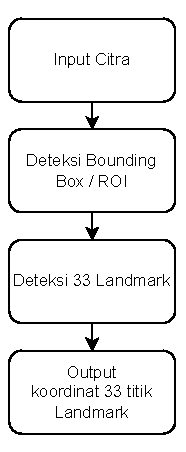
\includegraphics[width=0.24\textwidth]{figure/BAB 3/alur pemrosesan Pose Landmark.pdf}  % Menyisipkan gambar dengan lebar setengah lebar teks
    \caption{Alur proses deteksi pose landmark.}  % Menambahkan keterangan gambar
    \label{fig:alur pose landmark}  % Menambahkan label untuk referensi
\end{figure}

Terdapat 2 proses utama yang akan dilakukan dalam \textit{Mediapipe Pose} dengan memanfaatkan \textit{Blazepose}. Pertama, \textit{Blazepose} akan mendeteksi keberadaan tubuh manusia dalam gambar dan menghasilkan output berupa \textit{Bounding box} (kotak pembatas) yang mengelilingi tubuh serta titik referensi seperti pusat tubuh dan orientasi tubuh. \textit{BlazePose} akan menentukan \textit{Region of Interest} (ROI) yang berfokus pada area tubuh manusia dalam citra. Kedua, \textit{BlazePose} akan mendeteksi 33 titik koordinat (\textit{landmark}) dari tubuh manusia dalam ROI. 

\begin{figure}[htbp]  % 'h' menunjukkan gambar akan diletakkan di sekitar posisi ini
    \centering  % Gambar dipusatkan
    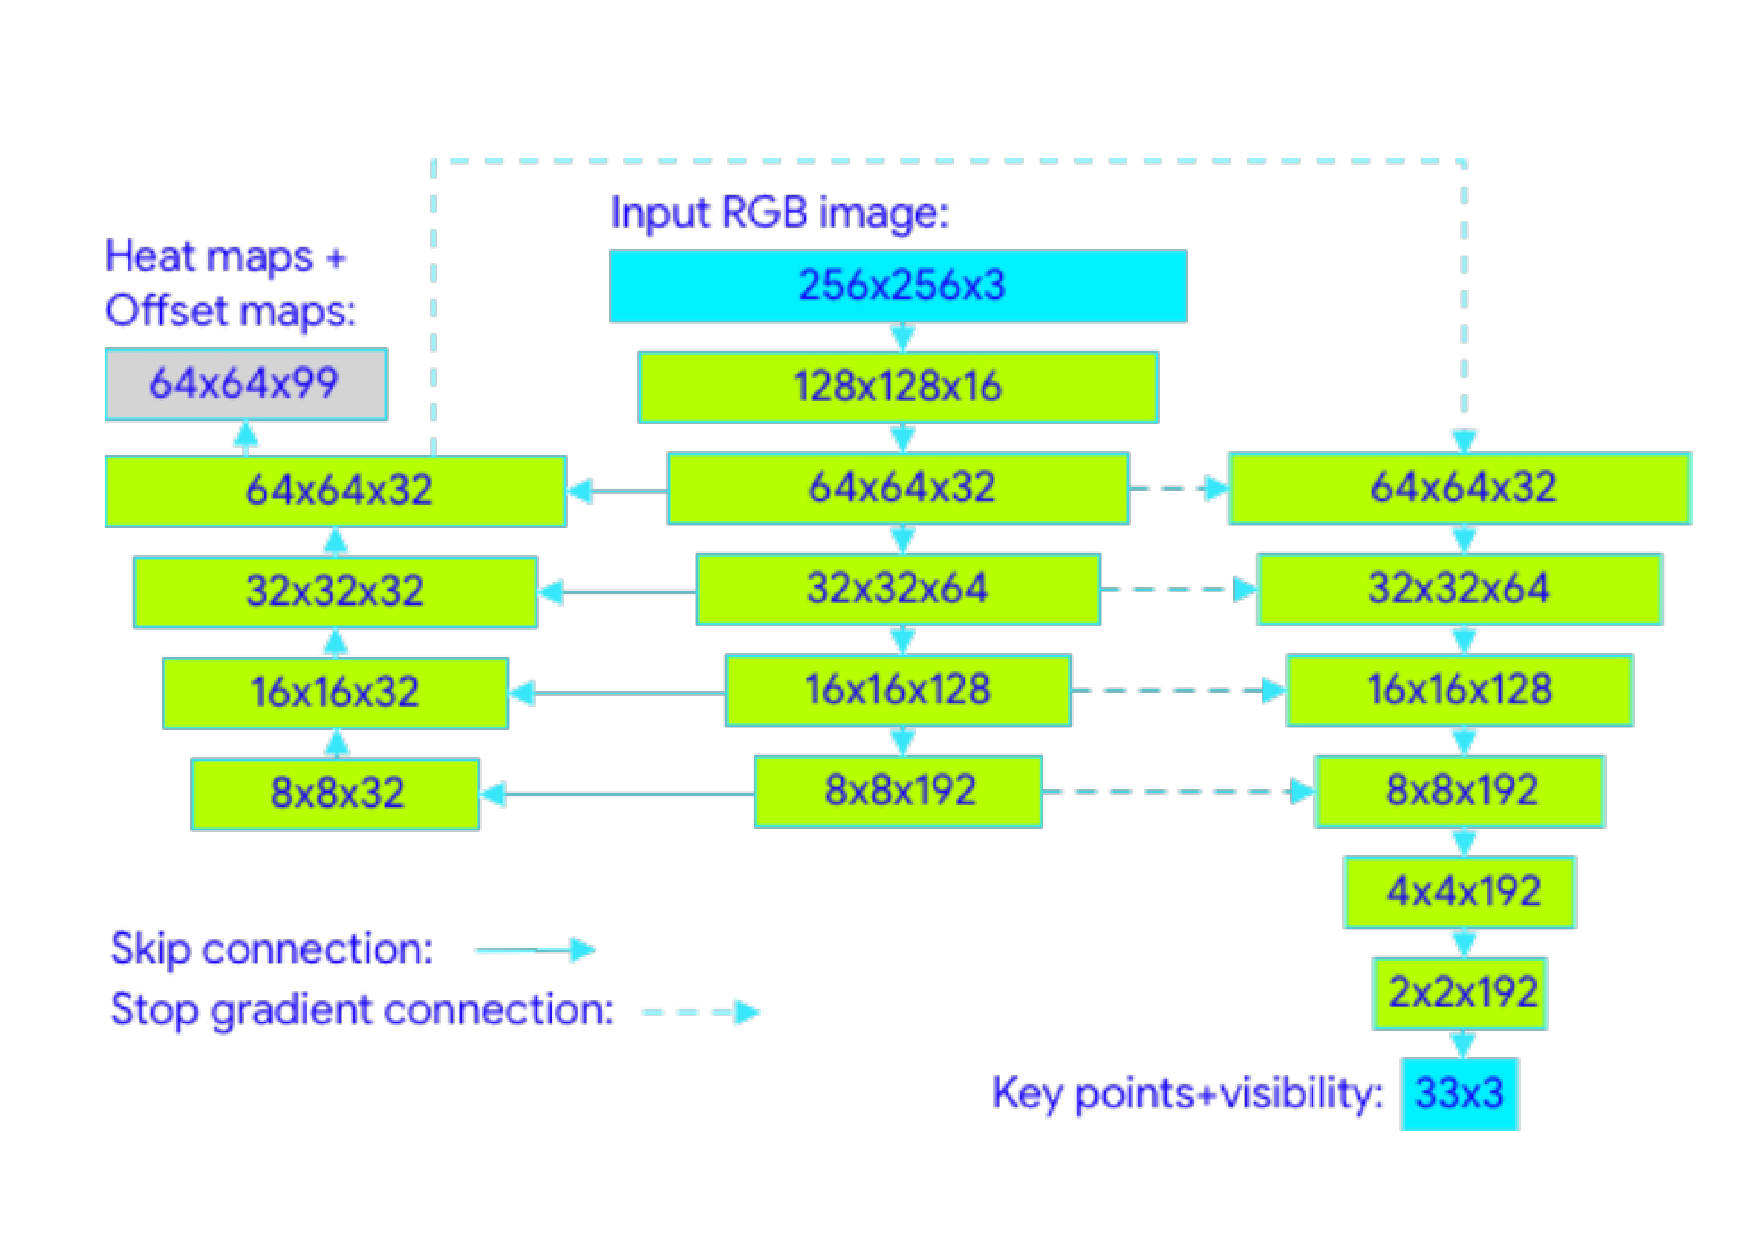
\includegraphics[width=0.8\textwidth]{figure/BAB 3/artisektur mediapipe pose.pdf}  % Menyisipkan gambar dengan lebar setengah lebar teks
    \caption{Arsitektur jaringan BlazePose \cite{bazarevsky2020}.}  % Menambahkan keterangan gambar
    \label{fig:arsitektur mediapipe}  % Menambahkan label untuk referensi
\end{figure}

Arsitektur jaringan \textit{BlazePose} menggunakan pendekatan kombinasi antara \textit{heatmap}, \textit{offset}, dan \textit{regression} untuk meningkatkan akurasi dan efisiensi dalam mendeteksi pose tubuh, seperti yang terlihat pada Gambar \ref{fig:arsitektur mediapipe}. Proses dimulai dengan menerima input citra RGB dengan dimensi 256x256x3 yang telah diproses secara otomatis dalam \textit{framework Mediapipe Pose,} tahapan awal dalam pipeline menyediakan proposal penyelarasan tubuh (\textit{person alignment}), yang membantu model dalam memfokuskan perhatian pada area tubuh yang relevan. Kemudian lapisan \textit{heatmap} hanya digunakan pada masa pelatihan model \textit{BlazePose} untuk mengarahkan proses pembelajaran dengan memberikan peta probabilitas yang menunjukkan kemungkinan posisi setiap \textit{landmark}, sementara \textit{offset loss} digunakan untuk mengoreksi perbedaan antara prediksi dan lokasi yang sebenarnya \cite{bazarevsky2020}.\par

Namun Pada saat ini, lapisan output yang terkait dengan \textit{heatmap} dan \textit{offset} dihapus karena model sudah menyelesaikan pelatihan dan masuk pada tahap inferensi, sehingga hanya jaringan \textit{regression} yang digunakan untuk memperkirakan titik koordinat (\textit{landmark}) dengan dimensi 33x3. Jaringan ini memanfaatkan \textit{skip-connections} di seluruh tahap untuk menggabungkan fitur tingkat tinggi dan rendah, memungkinkan model untuk menangkap informasi penting dari berbagai tingkat kompleksitas \cite{bazarevsky2020}. Berdasarkan struktur ini, \textit{BlazePose} berhasil mendeteksi pose \textit{landmark} tubuh manusia dengan akurasi tinggi, meskipun pada perangkat dengan sumber daya terbatas.\par

% \begin{figure}[htbp]  % 'h' menunjukkan gambar akan diletakkan di sekitar posisi ini
%     \centering  % Gambar dipusatkan
%     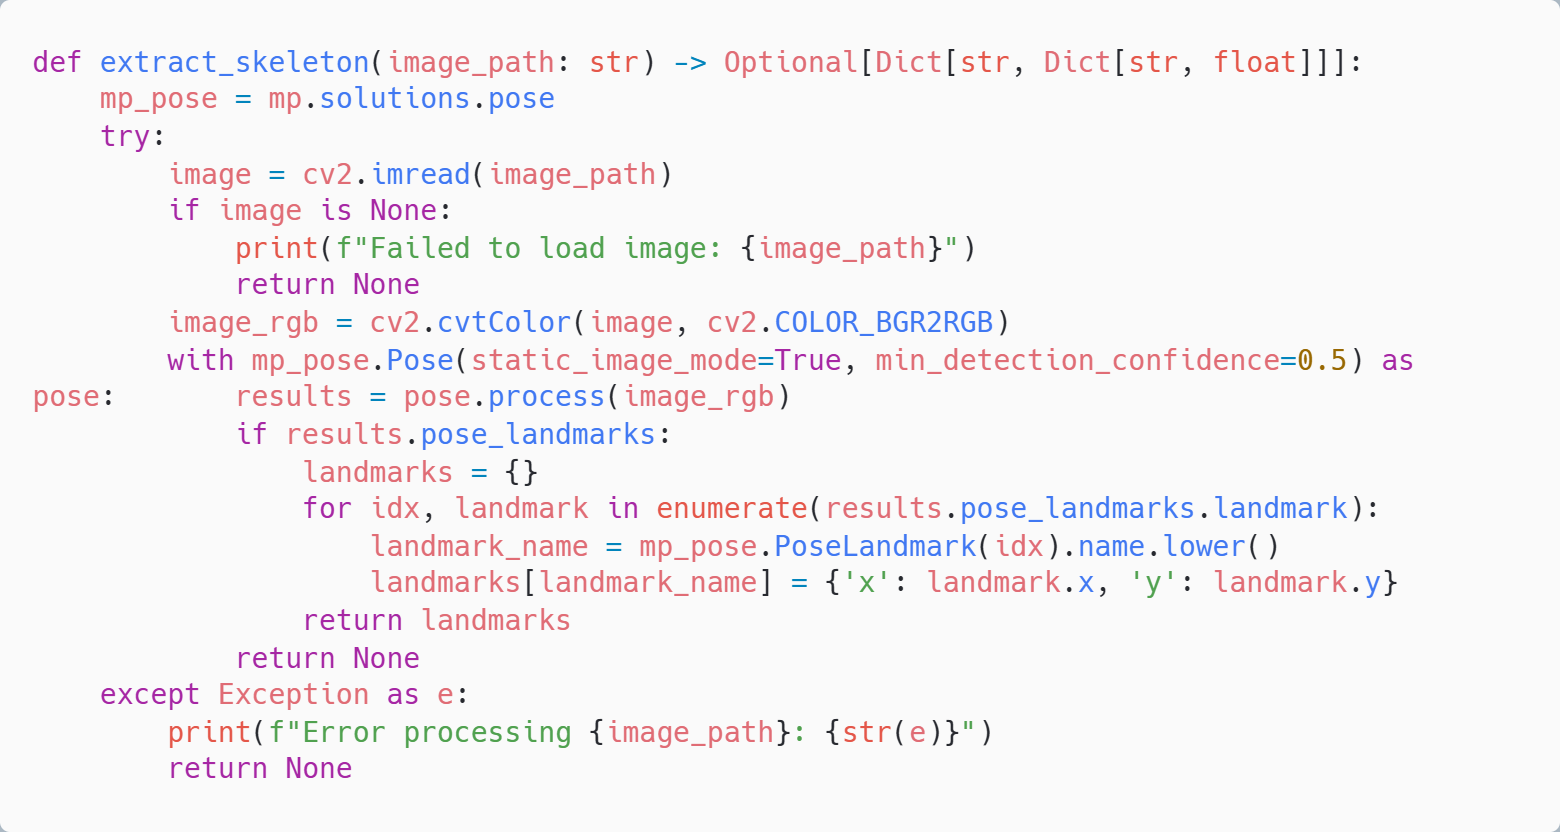
\includegraphics[width=1\textwidth]{images/extract_skeleton.png}  % Menyisipkan gambar dengan lebar setengah lebar teks
%     \caption{Kode ekstrak \textit{skeleton} dari citra}  % Menambahkan keterangan gambar
%     \label{fig:kode ekstrak skeleton}  % Menambahkan label untuk referensi
% \end{figure}

\begin{lstlisting}[caption={Ekstrak \textit{skeleton} dari citra}, label={kode:ekstrak skeleton}]
def extract_skeleton(image_path: str) -> Optional[Dict[str, Dict[str, float]]]:
    mp_pose = mp.solutions.pose
    
    try:
        # Read image
        image = cv2.imread(image_path)
        if image is None:
            print(f"Failed to load image: {image_path}")
            return None
            
        # Convert BGR to RGB
        image_rgb = cv2.cvtColor(image, cv2.COLOR_BGR2RGB)
        
        # Initialize pose detection
        with mp_pose.Pose(static_image_mode=True, min_detection_confidence=0.5) as pose:
            # Process image
            results = pose.process(image_rgb)
            
            if results.pose_landmarks:
                # Extract landmarks as dictionary
                landmarks = {}
                for idx, landmark in enumerate(results.pose_landmarks.landmark):
                    landmark_name = mp_pose.PoseLandmark(idx).name.lower()
                    landmarks[landmark_name] = {
                        'x': landmark.x,
                        'y': landmark.y,
                        'z': landmark.z
                    }
                return landmarks
            
            return None
\end{lstlisting}

\vspace{10pt}

Rancangan Program deteksi 33 \textit{pose landmark} menggunakan \textit{Mediapipe} dari citra terlihat pada Kode \ref{kode:ekstrak skeleton} dengan Fungsi \textit{extract\_skeleton} berperan sebagai inti deteksi pose. Fungsi ini membaca citra, mengonversi ruang warna dari BGR ke RGB agar sesuai dengan ekspektasi \textit{MediaPipe}, lalu menjalankan \textit{MediaPipe Pose} pada \textit{static\_image\_mode=True} sehingga setiap citra diperlakukan independen tanpa temporal smoothing antar frame untuk pipeline prapemrosesan berbasis citra. Ambang \textit{min\_detection\_confidence=0.5} dipilih sebagai kompromi antara \textit{recall} dan \textit{precision} karena dianggap cukup rendah untuk menangkap pose pada citra yang tidak ideal, misal sedikit blur atau \textit{occlusion} ringan, tetapi tetap membatasi \textit{false positives}. 


\begin{figure}[htbp]  % 'h' menunjukkan gambar akan diletakkan di sekitar posisi ini
    \centering  % Gambar dipusatkan
    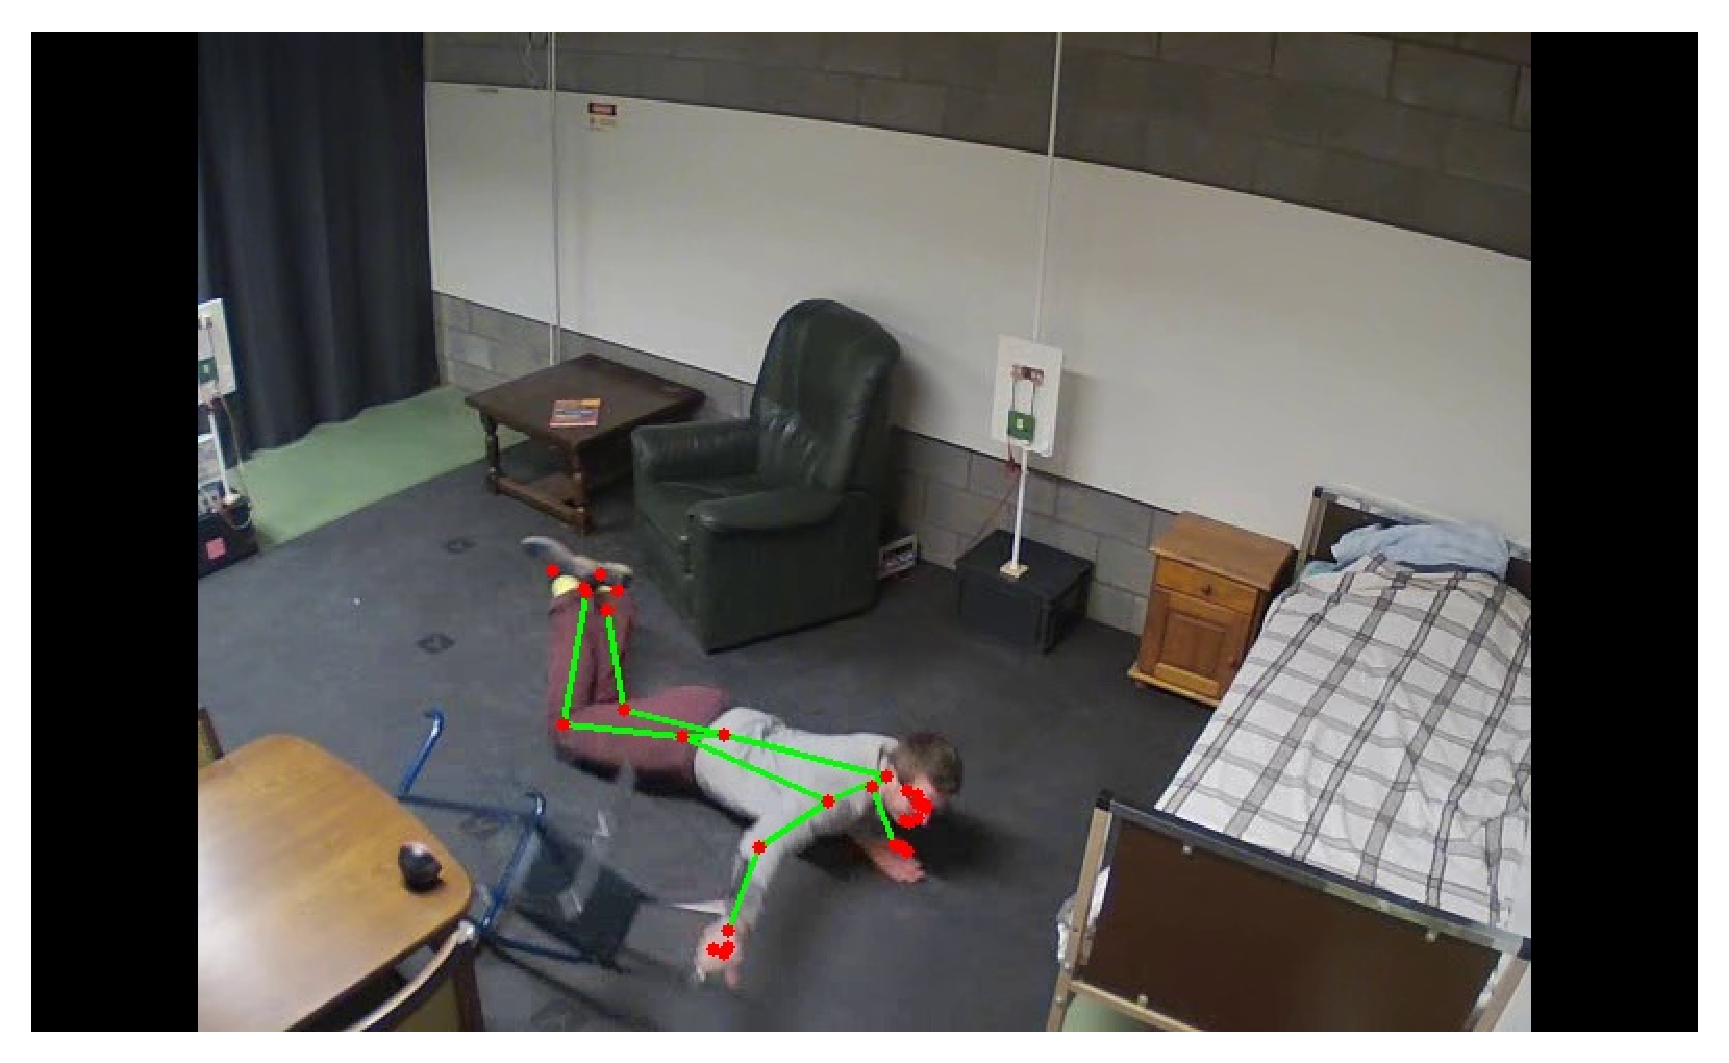
\includegraphics[width=0.7\textwidth, trim=3.5cm 0 3.5cm 0, clip]{figure/BAB 3/contoh deteksi landmark.pdf}  % Menyisipkan gambar dengan lebar setengah lebar teks
    \caption{\textit{Preview} hasil deteksi \textit{landmark} terhadap citra.}  % Menambahkan keterangan gambar
    \label{fig:contoh preview landmark}  % Menambahkan label untuk referensi
\end{figure}

Contoh \textit{preview} hasil deteksi \textit{landmark} dalam citra dapat dilihat pada Gambar \ref{fig:contoh preview landmark}. Setiap \textit{landmark} memiliki atribut x, y, dan z, di mana atribut x dan y menggambarkan posisi landmark terhadap sumbu simetri dalam citra, sementara atribut z menggambarkan kedalaman (3D) terhadap \textit{midpoint} dengan titik ukurnya berada pada area pinggul. Jika semakin kecil nilai z maka seakan-akan \textit{landmark} tersebut lebih dekat ke kamera. Seluruh \textit{landmark} yang berhasil dideteksi dalam masing-masing citra akan disimpan dalam file \textit{JSON} secara terpisah. Contoh data yang telah disimpan dapat dilihat pada Gambar \ref{fig:contoh landmark json}.\par

\begin{figure}[htbp]  % 'h' menunjukkan gambar akan diletakkan di sekitar posisi ini
    \centering  % Gambar dipusatkan
    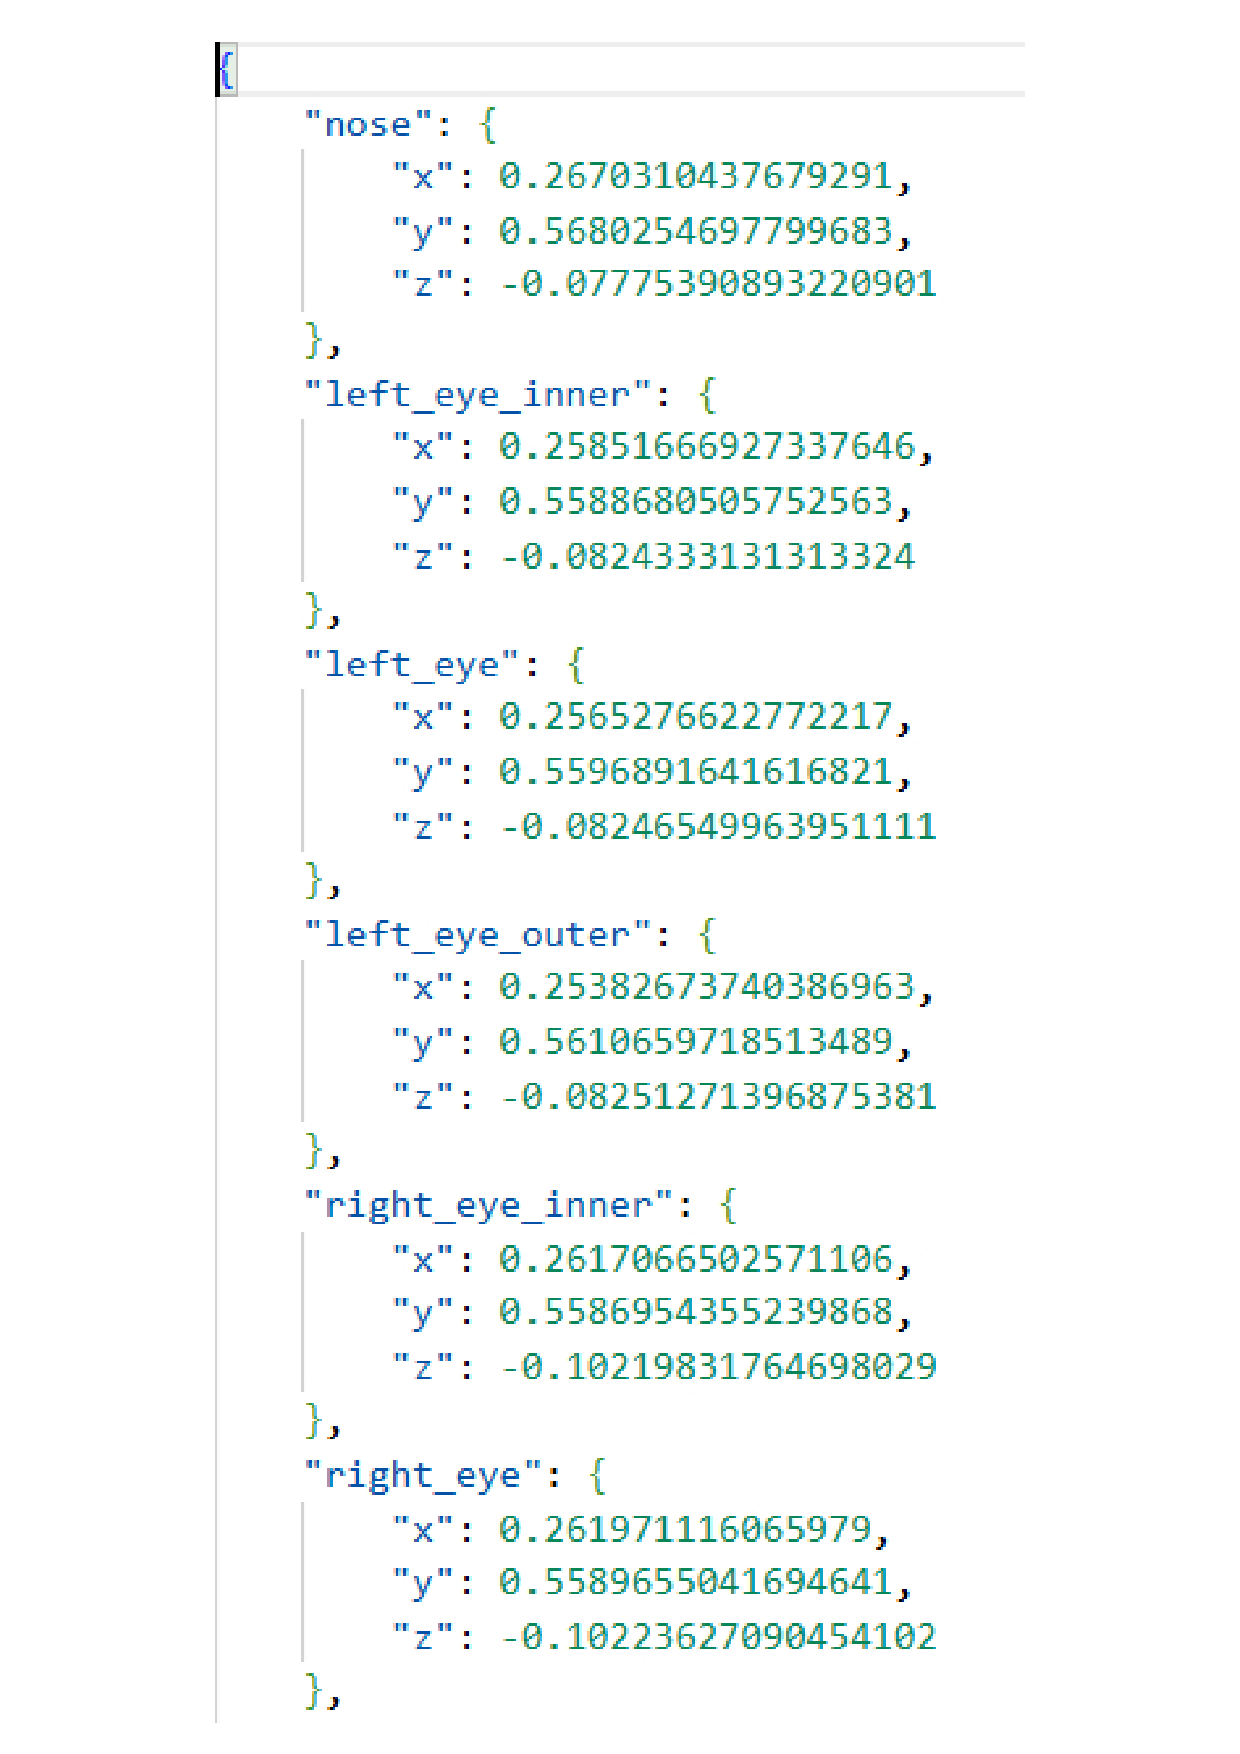
\includegraphics[width=0.45\textwidth]{figure/BAB 3/contoh data pose landmark.pdf} 
    \caption{Contoh data \textit{pose landmark}.}  % Menambahkan keterangan gambar
    \label{fig:contoh landmark json}  % Menambahkan label untuk referensi
\end{figure}


\subsubsection{Konversi \textit{Pose Landmark} Ke Graf}
\label{III.konversi landmark ke graf}

Setelah mendapatkan 33 \textit{landmark} dari masing-mmasing citra, data tersebut harus dikonversi terlebih dahulu menjadi format graf, karena model GCN memerlukan representasi data dalam bentuk graf untuk memproses hubungan antar node. Konversi ini melibatkan transformasi data menjadi tensor yang mencakup informasi \textit{node} dan \textit{edge}. Kemudian data tersebut dapat digunakan untuk pelatihan dan prediksi dengan model GCN. Alur konversinya dapat dilihat pada Gambar \ref{fig:alur konversi landmark graf}. \par

\begin{figure}[htbp]  % 'h' menunjukkan gambar akan diletakkan di sekitar posisi ini
    \centering  % Gambar dipusatkan
    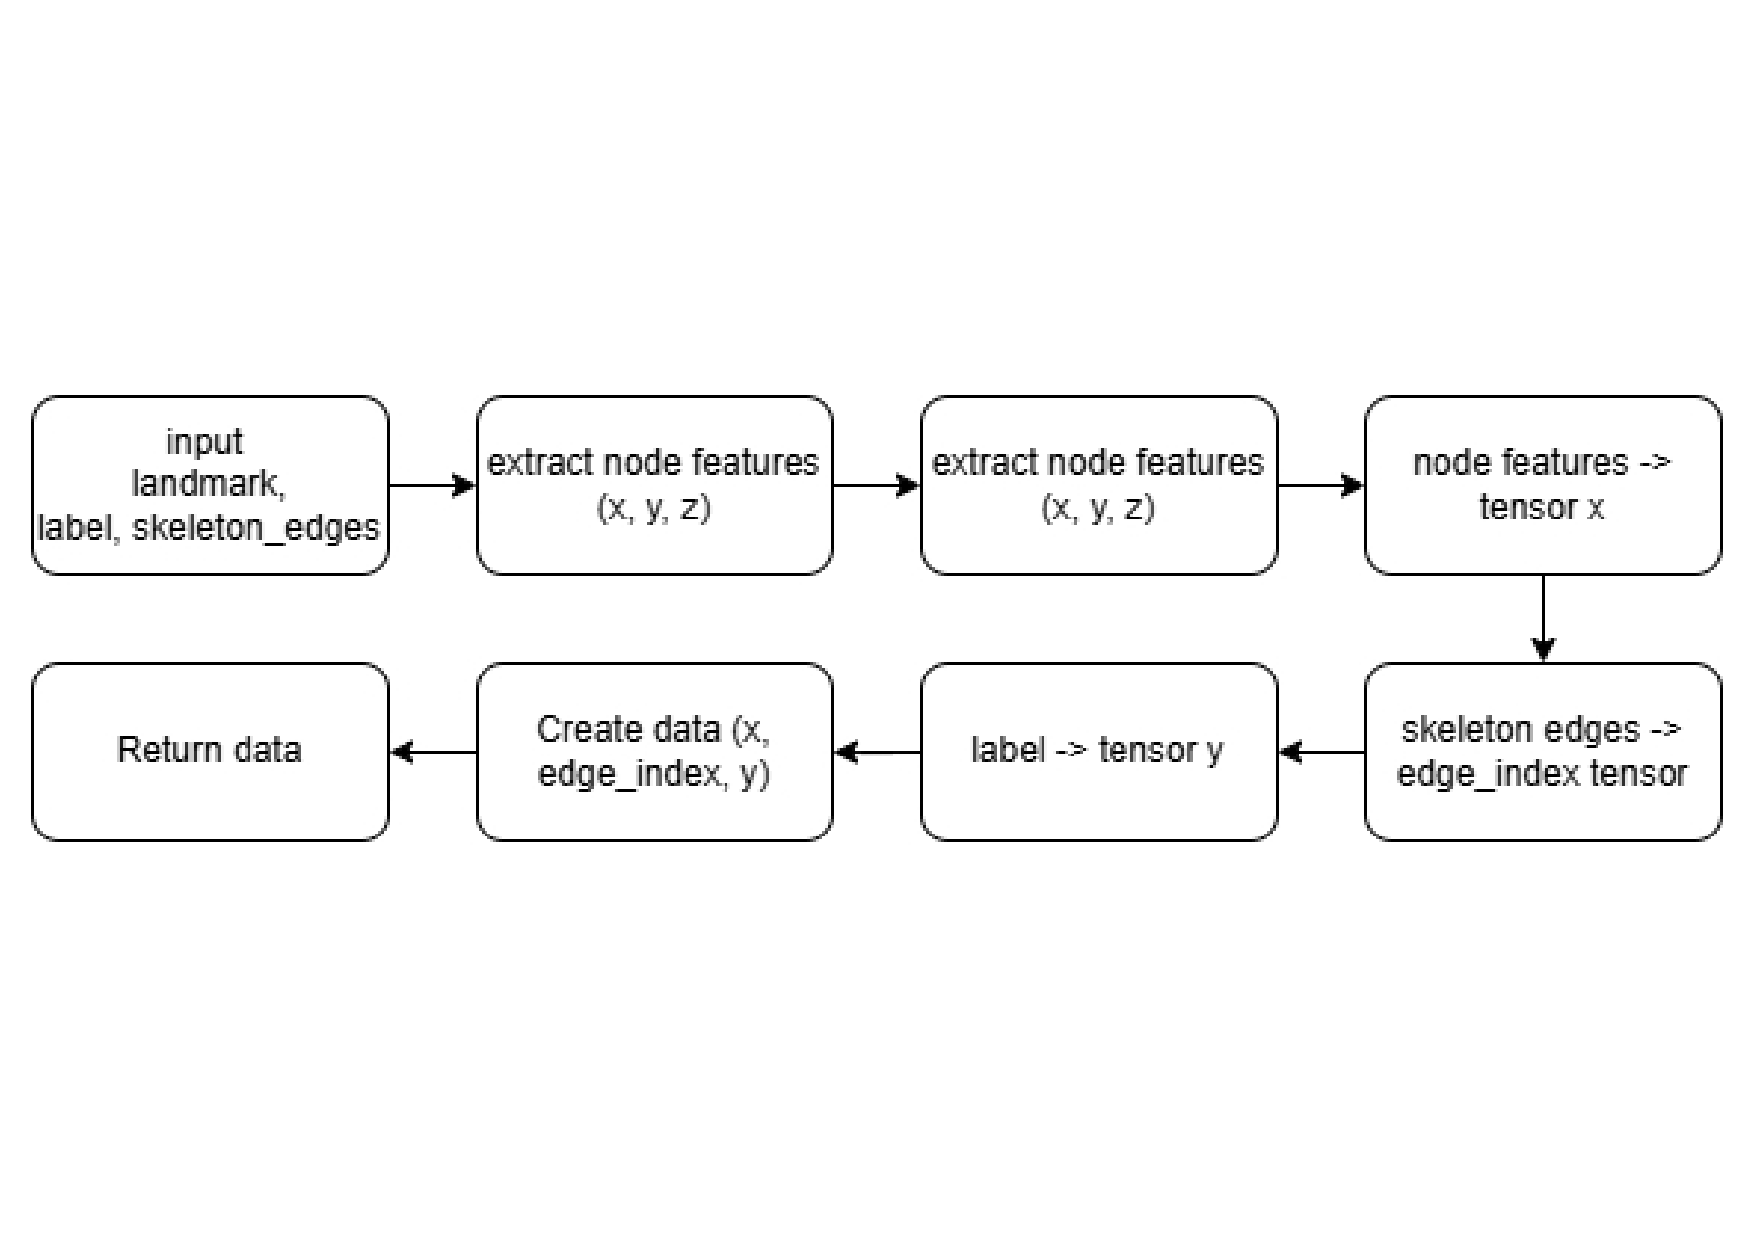
\includegraphics[width=1\textwidth]{figure/BAB 3/konversi pose landmark ke graf.pdf} 
    \caption{Alur konversi data \textit{pose landmark} ke data graf.}  % Menambahkan keterangan gambar
    \label{fig:alur konversi landmark graf}  % Menambahkan label untuk referensi
\end{figure}

Alur konversi \textit{pose landmark} ke graf dimulai dengan menerima input berupa data \textit{landmark}, label, dan \textit{skeleton edges}. \textit{Landmark} mewakili titik-titik pada tubuh manusia yang digunakan untuk menentukan pose, sementara \textit{skeleton edges} menggambarkan hubungan atau koneksi antar \textit{landmark } tersebut. Langkah pertama adalah mengekstrak fitur node untuk setiap \textit{landmark}, yang mencakup koordinat 3D (x, y, z). Fitur ini kemudian diubah menjadi sebuah tensor yang merepresentasikan posisi \textit{landmark} dalam ruang tiga dimensi. Setelah itu, \textit{skeleton edges}, yang menunjukkan hubungan antar \textit{landmark}, diubah menjadi tensor yang berisi indeks \textit{edge} (hubungan antar node). Data untuk graf kemudian dibuat dengan menggabungkan tensor yang berisi fitur \textit{node} (x), indeks \textit{edge} (\textit{edge\_index}), dan label (y) yang akan diprediksi. Label ini juga diubah menjadi tensor agar dapat diproses lebih lanjut. Setelah semua data dikonversi ke format tensor, data tersebut dikembalikan sebagai output yang siap digunakan dalam pemodelan graf atau analisis lebih lanjut, seperti yang terlihat pada Gambar \ref{fig:contoh data graf}. Dengan cara ini, data pose manusia dikonversi menjadi representasi graf yang siap diproses. \par

% \begin{figure}[H]  % 'h' menunjukkan gambar akan diletakkan di sekitar posisi ini
%     \centering  % Gambar dipusatkan
%     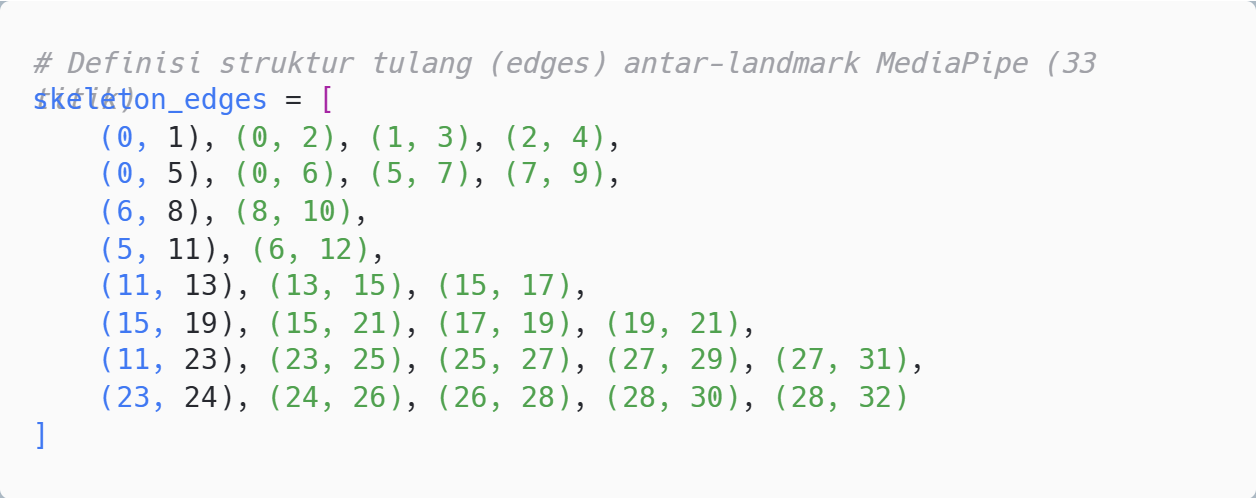
\includegraphics[width=1\textwidth]{images/skeleton_edges.png}  % Menyisipkan gambar dengan lebar setengah lebar teks
%     \caption{Kode inisialisasi struktur \textit{skeleton}}  % Menambahkan keterangan gambar
%     \label{fig:kode skeleton edges}  % Menambahkan label untuk referensi
% \end{figure}

\begin{lstlisting}[caption={Inisialisasi struktur \textit{skeleton}}, label={kode:skeleton edges}]
skeleton_edges = [
    (0, 1), (0, 2), (1, 3), (2, 4),
    (0, 5), (0, 6), (5, 7), (7, 9),
    (6, 8), (8, 10),
    (5, 11), (6, 12),
    (11, 13), (13, 15), (15, 17),
    (15, 19), (15, 21), (17, 19), (19, 21),
    (11, 23), (23, 25), (25, 27), (27, 29), (27, 31),
    (23, 24), (24, 26), (26, 28), (28, 30), (28, 32)
]
\end{lstlisting}

\vspace{10pt}

Pada Kode \ref{kode:skeleton edges} terlihat Daftar \textit{skeleton\_edges} yang mendefinisikan graf kerangka berdasarkan indeks \textit{landmark MediaPipe} (0–32). Tiap pasangan (u, v) menyatakan sisi terarah (yang kemudian ditranspos menjadi bentuk [2, E] untuk PyG) antara dua sendi, mencakup koneksi utama tubuh atas (mata, bahu, siku, pergelangan) hingga tubuh bawah (pinggul, lutut, pergelangan kaki, tumit, ujung kaki). Daftar ini menyandikan pengetahuan anatomi ke dalam struktur graf sehingga GCN dapat mengeksploitasi kedekatan struktural antartitik. \par

% \begin{figure}[H]  % 'h' menunjukkan gambar akan diletakkan di sekitar posisi ini
%     \centering  % Gambar dipusatkan
%     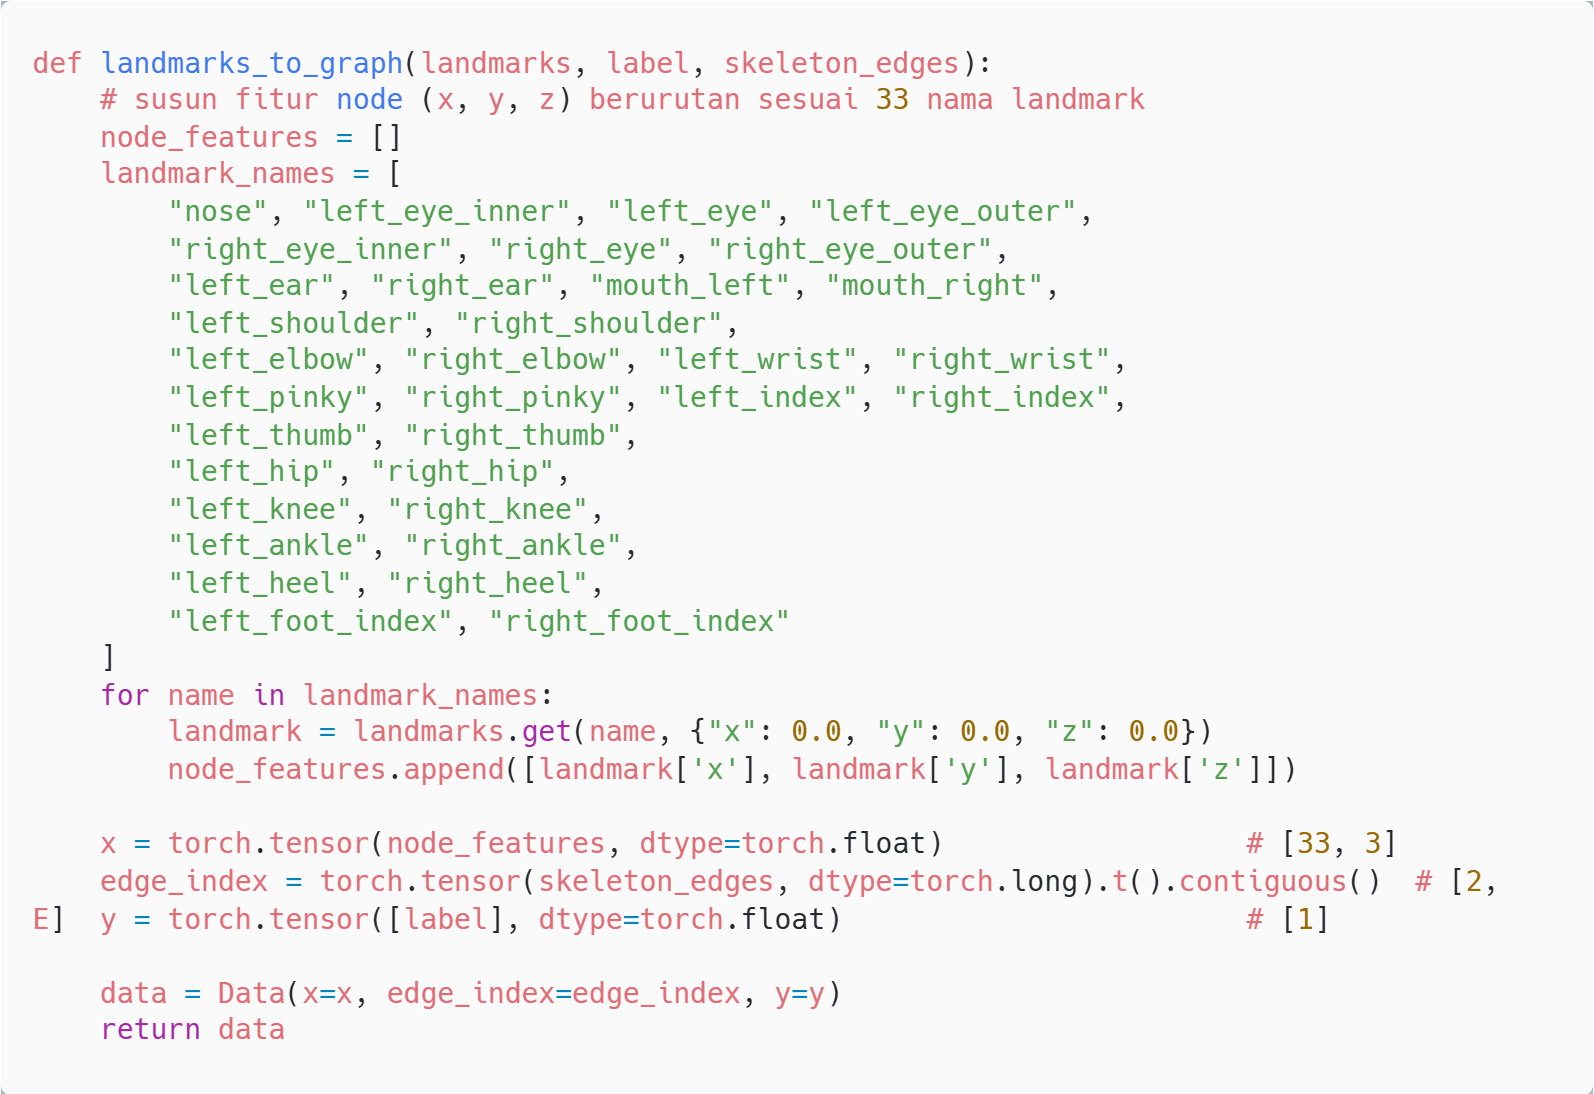
\includegraphics[width=1\textwidth]{images/landmark_to_graph.png}  % Menyisipkan gambar dengan lebar setengah lebar teks
%     \caption{Kode konversi \textit{skeleton} ke graf}  % Menambahkan keterangan gambar
%     \label{fig:kode konversi skeleton graf}  % Menambahkan label untuk referensi
% \end{figure}

\begin{lstlisting}[caption={konversi \textit{skeleton} ke graf}, label={kode:konversi skeleton graf}]
def landmarks_to_graph(landmarks, label, skeleton_edges):
    # Extract node features (x, y, z)
    node_features = []
    landmark_names = [
        "nose", "left_eye_inner", "left_eye", "left_eye_outer",
        "right_eye_inner", "right_eye", "right_eye_outer",
        "left_ear", "right_ear", "mouth_left", "mouth_right",
        "left_shoulder", "right_shoulder",
        "left_elbow", "right_elbow", "left_wrist", "right_wrist",
        "left_pinky", "right_pinky", "left_index", "right_index",
        "left_thumb", "right_thumb",
        "left_hip", "right_hip",
        "left_knee", "right_knee",
        "left_ankle", "right_ankle",
        "left_heel", "right_heel",
        "left_foot_index", "right_foot_index"
    ]
    
    for name in landmark_names:
        landmark = landmarks.get(name, {"x": 0.0, "y": 0.0, "z": 0.0}) # , "z": 0.0
        node_features.append([landmark['x'], landmark['y'], landmark['z']]) # , landmark['z']
    
    x = torch.tensor(node_features, dtype=torch.float)
    
    # Define edge_index based on skeleton_edges
    edge_index = torch.tensor(skeleton_edges, dtype=torch.long).t().contiguous()
    
    # Label
    y = torch.tensor([label], dtype=torch.float)
    
    # Create graph data
    data = Data(x=x, edge_index=edge_index, y=y)
    
    return data
\end{lstlisting}

\vspace{10pt}

Fungsi \textit{landmarks\_to\_graph} pada Kode \ref{kode:konversi skeleton graf} mengubah hasil deteksi pose menjadi graf \textit{PyTorch Geometric} (torch\_geometric.data.Data) yang siap untuk pelatihan GCN. Pertama, urutan \textit{landmark\_names} menegakkan indeks node yang konsisten (0–32), sehingga setiap sampel selalu menyusun fitur node [x, y, z] dalam urutan identik. Ini penting agar filter konvolusi graf melihat node yang sama di posisi yang sama antar-sampel. Tensor x berukuran [33, 3] memuat fitur koordinat 3 dimensi, sedangkan \textit{edge\_index} adalah indeks sisi [2, E] hasil \textit{t().contiguous()} agar kompatibel dengan kernel PyG. Label y dibuat sebagai tensor (1) bertipe float untuk klasifikasi biner. \par


\subsubsection{Pembagian \textit{K-Fold} Pada Data}

Tahap selanjutnya yaitu menerapkan teknik pembagian dataset \textit{K-Fold}. Ini adalah teknik yang bertujuan untuk membagi dataset menjadi beberapa bagian yang disebut "\textit{fold}", artinya teknik ini dapat membuat sebanyak~$k$ variasi subset data jatuh dan tidak jatuh untuk membantu generalisasi model sekaligus mengurangi potensi \textit{overfitting}. Namun terdapat Konsekuensi dimana siklus pelatihan membutuhkan waktu dan sumber daya komputasi lebih besar dibandingkan skema pembagian data pelatihan konvensional. Selain itu terdapat pertimbangan lain, yaitu Jika nilai~$k$ terlalu besar, pembagian data menjadi lebih banyak lipatan akan mengakibatkan ukuran data di setiap lipatan menjadi lebih kecil, yang dapat menghasilkan estimasi varians yang lebih tinggi, terutama jika dataset tidak cukup besar. Sebaliknya, jika nilai~$k$ terlalu kecil, maka risiko bias terhadap estimasi kesalahan model dapat meningkat \cite{Hadjisolomou2021}.

Penggunaan K-fold dengan K = 5 telah terbukti menjadi pilihan yang efektif dalam banyak aplikasi dan masih merupakan "standar yang baik" dalam banyak model. Hal ini memberi keseimbangan yang baik antara bias dan varians, memungkinkan efisiensi waktu komputasi yang lebih baik daripada pengaturan yang lebih tinggi \cite{Hadjisolomou2021}. Oleh karena itu, penelitian ini ditetapkan $k = 5$. Langkah pertama penerapan K-fold adalah mengelompokkan dataset \textit{pose landmark} berdasarkan \textit{prefix} folder—yang merepresentasikan sesi perekaman—agar data dari subjek yang sama tidak tercampur antara pelatihan dan validasi. Daftar \textit{prefix} tersebut kemudian dibagi ke dalam lima \textit{fold} proporsional memakai fungsi \texttt{KFold} dari \textit{scikit-learn}. \par

\begin{figure}[htbp]  % 'h' menunjukkan gambar akan diletakkan di sekitar posisi ini
    \centering  % Gambar dipusatkan
    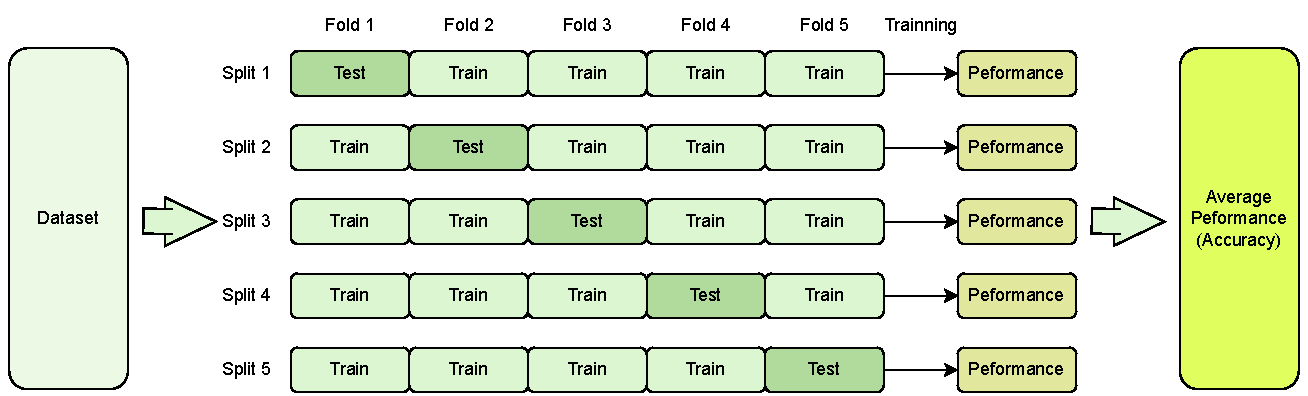
\includegraphics[width=1\textwidth]{figure/BAB 3/K-fold.pdf}  % Menyisipkan gambar dengan lebar setengah lebar teks
    \caption{Pembagian dataset menggunakan \textit{5-Fold}}  % Menambahkan keterangan gambar
    \label{fig:k-fold}  % Menambahkan label untuk referensi
\end{figure}

Illustrasi pembagian dataset dengan teknik k-fold dapat dilihat pada Gambar \ref{fig:k-fold}. Keseluruhan dataset jatuh dan tidak jatuh dibagi menjadi 5 fold dengan tiap fold berisi 20\% dari keseluruhan data. Lalu 5 fold tersebut disusun dengan variasi 5 Split yang masing-masing terdiri dari 80\% data pelatihan dan 20\% data evaluasi. Setiap 1 kali iterasi dilakukan proses pelatihan sebanyak 5 kali mengggunakan 5 \textit{fold} yang berbeda, dengan setiap \textit{fold} melatih model baru, artinya dalam pelatihan Kfold ini ada 5 model yang telah dilatih menggunakan 5 variasi pembagian dataset.\par

% \begin{figure}[htbp]
%     \centering  % Gambar dipusatkan
%     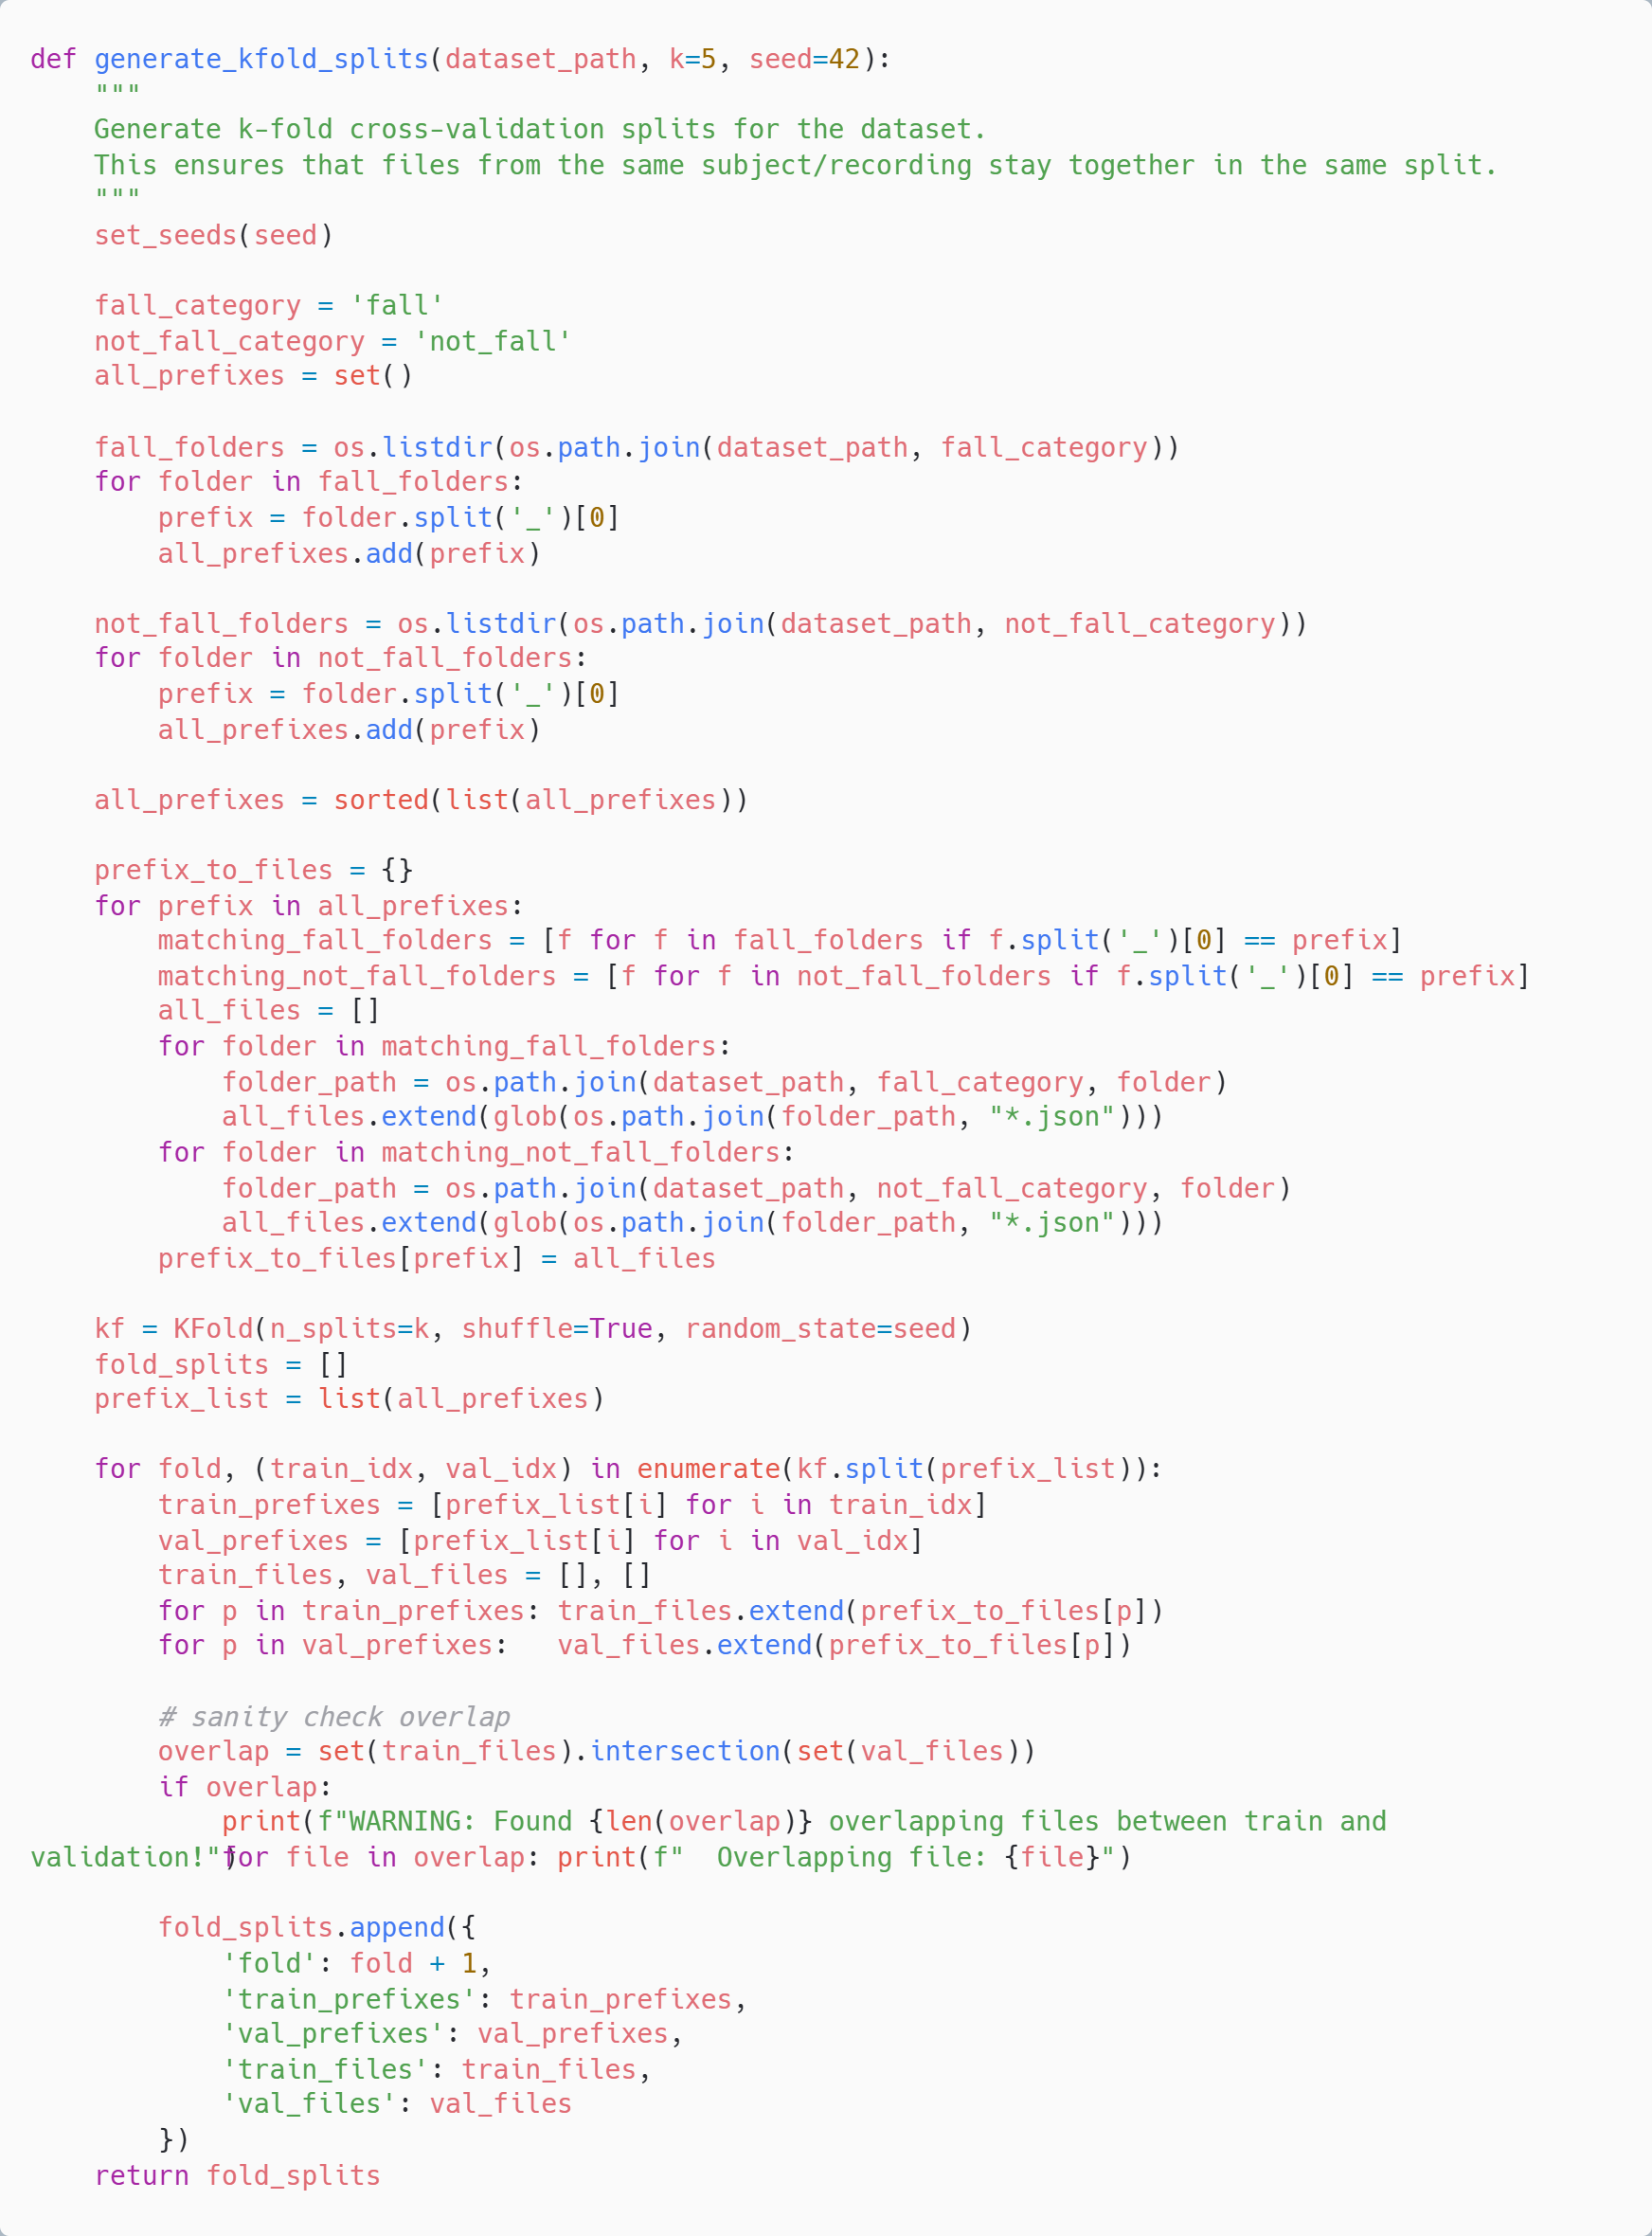
\includegraphics[width=1\textwidth]{images/generate_kfold_splits.png}  % Menyisipkan gambar dengan lebar setengah lebar teks
%     \caption{Kode membuat pembagian K-Fold}  % Menambahkan keterangan gambar
%     \label{fig:kode generate k-fold}  % Menambahkan label untuk referensi
% \end{figure}


\begin{lstlisting}[caption={Membuat pembagian K-Fold}, label={kode:generate k-fold}]
def generate_kfold_splits(dataset_path, k=5, seed=42):
    """
    Generate k-fold cross-validation splits for the dataset.
    This ensures that files from the same subject/recording stay together in the same split.
    
    Args:
        dataset_path (str): Path to the dataset root
        k (int): Number of folds
        seed (int): Random seed for reproducibility
        
    Returns:
        list: List of dictionaries containing train and val files for each fold
    """
    set_seeds(seed)
    
    fall_category = 'fall'
    not_fall_category = 'not_fall'
    
    # Get all group prefixes from the folder names
    all_prefixes = set()
    
    # Get all fall folders
    fall_folders = os.listdir(os.path.join(dataset_path, fall_category))
    for folder in fall_folders:
        prefix = folder.split('_')[0]
        all_prefixes.add(prefix)
    
    # Get all not_fall folders
    not_fall_folders = os.listdir(os.path.join(dataset_path, not_fall_category))
    for folder in not_fall_folders:
        prefix = folder.split('_')[0]
        all_prefixes.add(prefix)
    
    # Convert to sorted list for deterministic behavior
    all_prefixes = sorted(list(all_prefixes))
    
    print(f"Found {len(all_prefixes)} unique prefixes: {all_prefixes}")
    
    # Create a mapping from prefix to all files in that group
    prefix_to_files = {}
    
    # Process fall files
    for prefix in all_prefixes:
        matching_fall_folders = [folder for folder in fall_folders if folder.split('_')[0] == prefix]
        matching_not_fall_folders = [folder for folder in not_fall_folders if folder.split('_')[0] == prefix]
        
        all_files = []
        
        # Get all fall files for this prefix
        for folder in matching_fall_folders:
            folder_path = os.path.join(dataset_path, fall_category, folder)
            json_files = glob(os.path.join(folder_path, "*.json"))
            all_files.extend(json_files)
        
        # Get all not_fall files for this prefix
        for folder in matching_not_fall_folders:
            folder_path = os.path.join(dataset_path, not_fall_category, folder)
            json_files = glob(os.path.join(folder_path, "*.json"))
            all_files.extend(json_files)
        
        prefix_to_files[prefix] = all_files
        print(f"Prefix {prefix}: {len(all_files)} files")
    
    # Initialize k-fold cross-validation on the prefixes, not individual files
    kf = KFold(n_splits=k, shuffle=True, random_state=seed)
    
    # Generate splits based on prefixes
    fold_splits = []
    
    # Convert prefixes to list for sklearn's KFold
    prefix_list = list(all_prefixes)
    
    for fold, (train_idx, val_idx) in enumerate(kf.split(prefix_list)):
        train_prefixes = [prefix_list[i] for i in train_idx]
        val_prefixes = [prefix_list[i] for i in val_idx]
        
        train_files = []
        val_files = []
        
        # Collect all files for train and val splits based on their prefixes
        for prefix in train_prefixes:
            train_files.extend(prefix_to_files[prefix])
        
        for prefix in val_prefixes:
            val_files.extend(prefix_to_files[prefix])
        
        # Check for any overlap between train and validation files
        train_set = set(train_files)
        val_set = set(val_files)
        overlap = train_set.intersection(val_set)
        if overlap:
            print(f"WARNING: Found {len(overlap)} overlapping files between train and validation!")
            for file in overlap:
                print(f"  Overlapping file: {file}")
        
        # Add split to result
        fold_splits.append({
            'fold': fold + 1,
            'train_prefixes': train_prefixes,
            'val_prefixes': val_prefixes,
            'train_files': train_files,
            'val_files': val_files
        })
        
        print(f"Fold {fold+1}:")
        print(f"  Train: {len(train_prefixes)} prefixes, {len(train_files)} files")
        print(f"  Validation: {len(val_prefixes)} prefixes, {len(val_files)} files")
    
    return fold_splits
\end{lstlisting}

\vspace{10pt}

Program fungsi \textit{generate\_kfold\_splits} Pada Kode \ref{kode:generate k-fold} membangun skema validasi silang berbasis grup untuk mencegah kebocoran data antar video. Prinsipnya yaitu nama folder di dalam data skeleton seperti diasumsikan memiliki prefix (bagian sebelum \_) yang merepresentasikan identitas subjek atau sesi rekaman. Fungsi ini mengumpulkan seluruh prefix dari kedua kategori, memetakan setiap prefix ke semua berkas .json (hasil ekstraksi \textit{landmark}), lalu menjalankan pembagian K-Fold di level prefix. Dengan begitu, seluruh file milik satu prefix akan selalu jatuh ke satu split (train atau val), sehingga model tidak melihat data yang sama di dua subset berbeda. Prosedur juga menyertakan \textit{sanity check} untuk mendeteksi tumpang tindih file. Jika ada overlap, peringatan dicetak agar peneliti dapat meninjau struktur data. Penjabaran hasil akhirnya dapat dilihat pada Tabel \ref{tab:data k-fold}. \par


\subsection{Perancangan Model GCN} \label{III.perancangan GCN}
Pada tahap ini dipaparkan rancangan pipeline pembangunan model secara keseluruhan. Perancangan memanfaatkan Graph Convolutional Network (GCN) dengan arsitektur yang terinspirasi dari ResGCN untuk menangkap hubungan antar-node secara efektif melalui koneksi residual. Penyetelan model dilakukan dengan mengatur sejumlah hyperparameter kunci, meliputi jenis optimizer, learning rate, weight decay, batch size, dropout, jumlah epoch, ukuran hidden channel, serta pengaktifan residual untuk memperoleh kinerja optimal. \par

\begin{figure}[htbp]  % 'h' menunjukkan gambar akan diletakkan di sekitar posisi ini
    \centering  % Gambar dipusatkan
    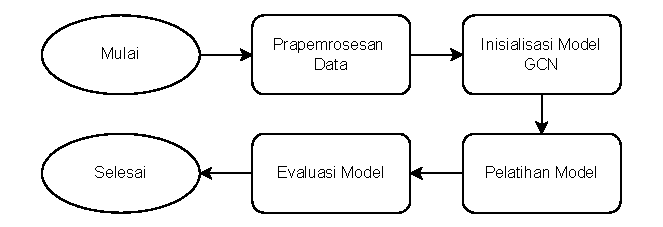
\includegraphics[width=0.9\textwidth]{figure/BAB 3/Diagram perancangan model gcn.pdf}  % Menyisipkan gambar dengan lebar setengah lebar teks
    \caption{Alur perancangan model}  % Menambahkan keterangan gambar
    \label{fig:Alur perancangan model}  % Menambahkan label untuk referensi
\end{figure}

Berdasarkan rancangan pada Gambar \ref{fig:Alur perancangan model}, alur perancangan model dimulai dari dataset awal berupa kumpulan video berlabel jatuh dan tidak jatuh yang harus diproses terlebih dahulu agar dapat digunakan dalam pelatihan model. Tahap prapemrosesan dilakukan dengan mengekstrak 30 citra dari setiap klip waktu pada tiap video sesuai panduan pada \textit{meta file}. Setiap citra kemudian diproses menggunakan inferensi \textit{MediaPipe Pose} untuk memperoleh rangka tubuh (\textit{skeleton}) yang memuat koordinat \textit{node} serta struktur \textit{edge}. Seluruh koordinat disimpan sebagai berkas JSON terpisah (satu JSON per citra). Dataset selanjutnya dibagi menggunakan skema \textit{5-Fold} guna menilai kualitas pelatihan model. Sebelum diproses lebih lanjut, data koordinat tersebut dikonversi ke representasi graf sehingga dapat diterima oleh model GCN. \par

Model klasifikasi berbasis GCN dilatih untuk tugas klasifikasi biner "jatuh atau tidak jatuh" pada tiap graf. Skema 5-fold digunakan untuk membagi data latih dan validasi dengan pengelompokan citra per video guna mencegah kebocoran identitas antar video. Selama pelatihan, digunakan \textit{Binary Cross-Entropy (BCE) loss} sebagai fungsi kerugian. Untuk menilai konsistensi dan efisiensi pembelajaran, pelatihan diulang sebanyak lima kali dengan inisialisasi ulang dan masing-masing dijalankan pada \textit{fold} yang berbeda. Evaluasi difokuskan pada metrik akurasi dan nilai \textit{loss} untuk menilai kemampuan model dalam memprediksi posisi jatuh dan tidak jatuh pada setiap citra. \par


\begin{figure}[htbp]  % 'h' menunjukkan gambar akan diletakkan di sekitar posisi ini
    \centering  % Gambar dipusatkan
    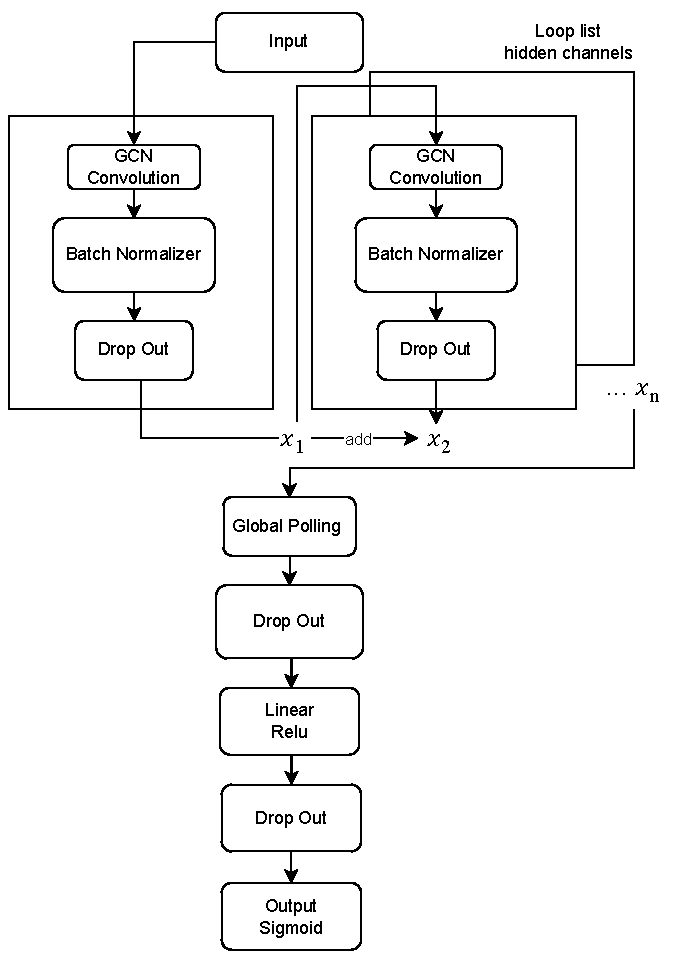
\includegraphics[width=0.8\textwidth]{figure/BAB 3/Arsitektur model GCN.pdf}  % Menyisipkan gambar dengan lebar setengah lebar teks
    \caption{Rancangan arsitektur model GCN.}  % Menambahkan keterangan gambar
    \label{fig:arsitektur model gcn}  % Menambahkan label untuk referensi
\end{figure}

Model GCN dirancang seperti yang terlihat pada Gambar \ref{fig:arsitektur model gcn}. Lapisan pertama menerima input data \textit{pose landmark} yang telah dikonversi menjadi representasi graf. Lalu Pada lapisan GCN \textit{Convolution}, data input melalui proses konvolusi dimana GCN bekerja dengan memperbarui fitur setiap node berdasarkan fitur tetangga sekitarnya, memungkinkan model untuk memanfaatkan struktur graf untuk membuat prediksi yang lebih baik. Setelah itu lapisan \textit{Batch Normalizer} digunakan untuk menormalkan output dari lapisan sebelumnya agar membantu mengurangi pergeseran distribusi data selama pelatihan, sehingga mempercepat proses pelatihan dan meningkatkan stabilitas model.\par

Lapisan \textit{Dropout} digunakan untuk mencegah overfitting dengan secara acak mematikan beberapa unit pada lapisan tersebut selama pelatihan. Ini membantu model untuk tidak terlalu bergantung pada fitur tertentu dan membuatnya lebih generalisasi. Lapisan \textit{Global Pooling} digunakan untuk mengurangi dimensi data setelah proses konvolusi, dengan cara mengambil informasi dari seluruh graf dan merangkum fitur-fitur penting dalam representasi yang lebih ringkas. Selanjutnya ditambahkan lapisan \textit{Linear} dengan aktivasi \textit{Relu}, bertugas untuk menghubungkan informasi yang telah diproses sebelumnya ke dalam bentuk representasi yang dapat digunakan untuk klasifikasi atau prediksi. Lapisan terakhir, \textit{fully connected} dengan fungsi aktivasi sigmoid, mengubah output model menjadi probabilitas yang dapat digunakan untuk klasifikasi dua kelas, yaitu jatuh atau tidak jatuh. \par

Dikembangkan program berbasis \textit{Class} agar dapat mewujudkan rancangan arsitektur model yang telah dijabarkan sebelumnya. Program inisialisasi komponen arsitektur tersebut dapat dilihat pada Kode \ref{kode:inisialisasi gcn}. Kemudian dibutuhkan inisialisasi proses untuk menentukan bagaimana pembelajaran model berlangsung secara \textit{forward}. Oleh karena itu dibuat fungsi \textit{forward propagation} seperti yang terlihat juga pada Kode \ref{kode:inisialisasi gcn}. Penjelasan lebih lengkap dapat dilihat pada Subbab \ref{IV.Perancangan}. \par
 
% \begin{figure}[htbp]  % 'h' menunjukkan gambar akan diletakkan di sekitar posisi ini
%     \centering  % Gambar dipusatkan
%     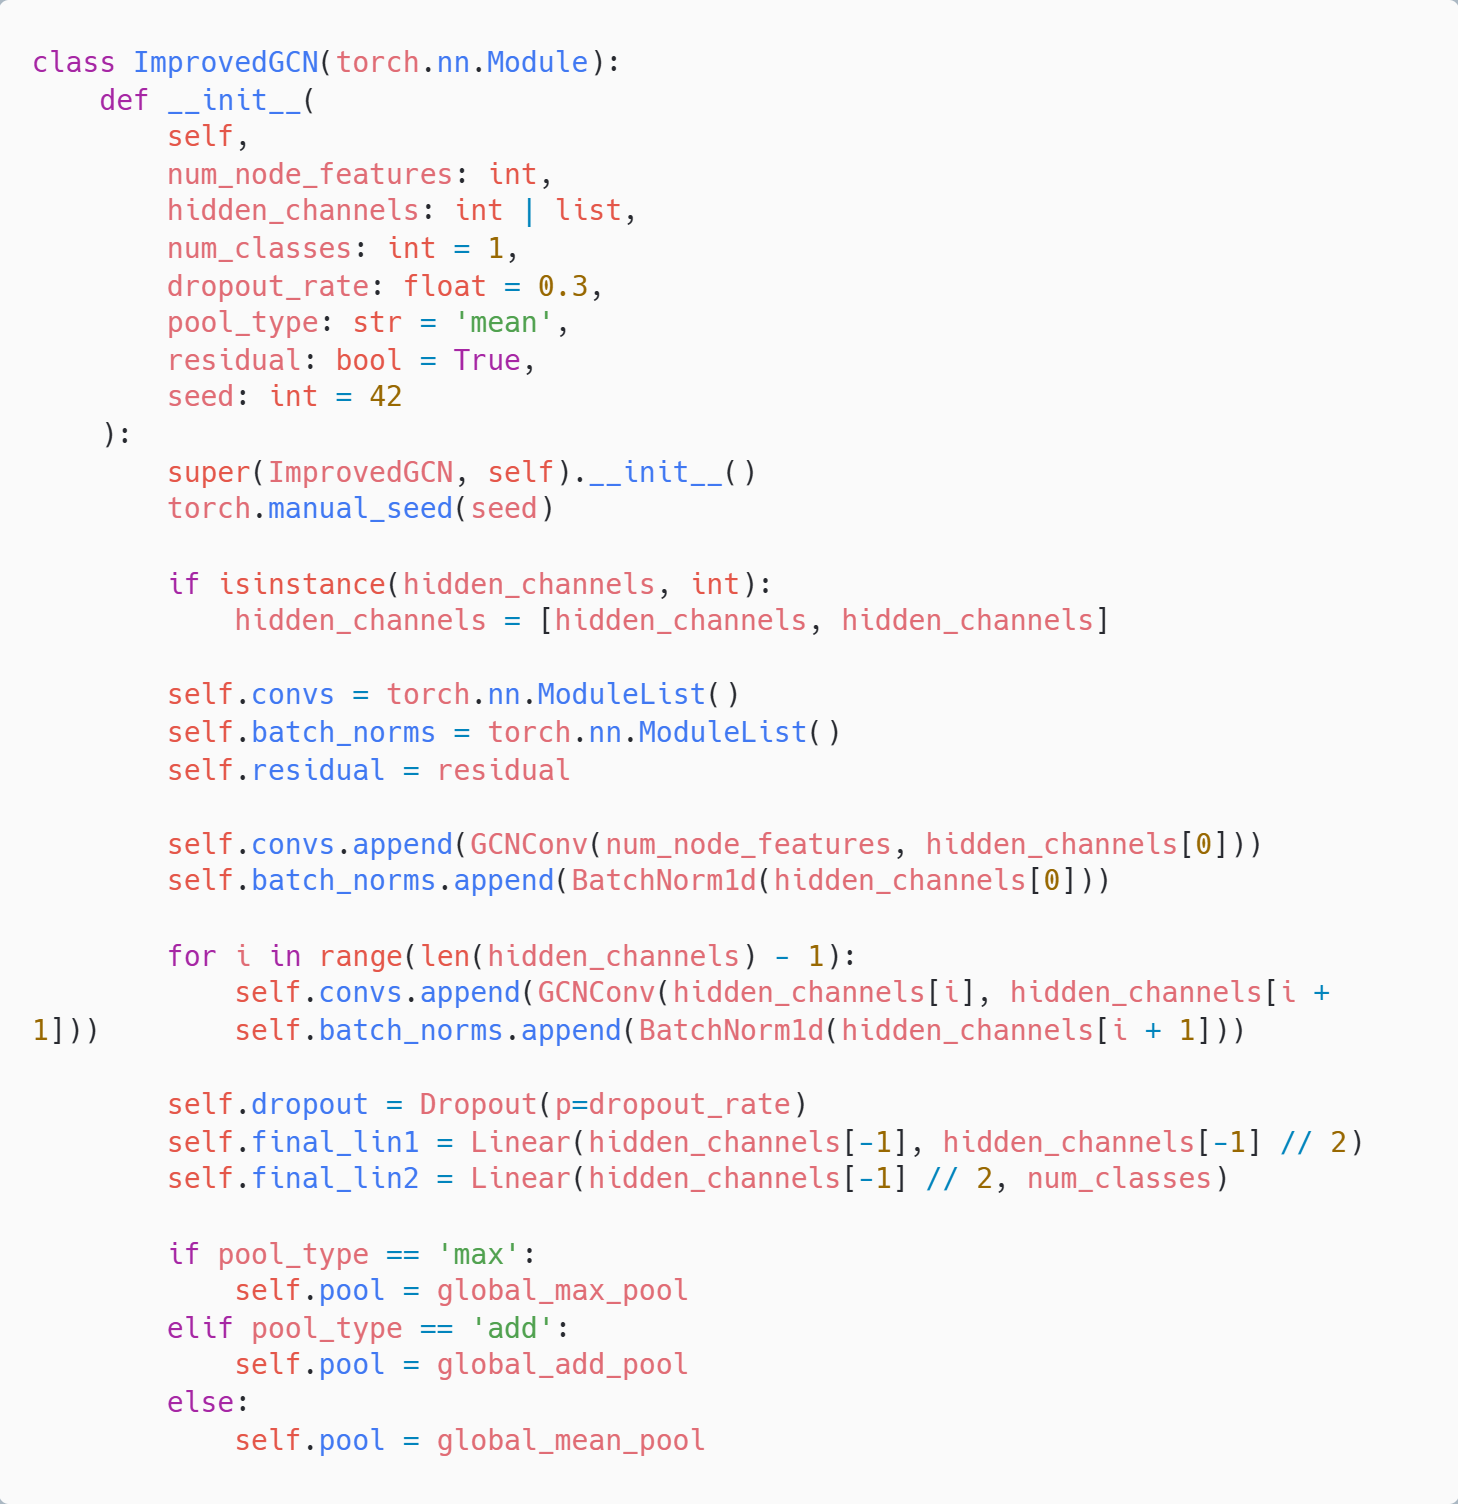
\includegraphics[width=1\textwidth]{images/class improved gcn.png}  % Menyisipkan gambar dengan lebar setengah lebar teks
%     \caption{Kode inisialisasi arsitektur model GCN}  % Menambahkan keterangan gambar
%     \label{fig:inisialisasi gcn}  % Menambahkan label untuk referensi
% \end{figure}

\begin{lstlisting}[caption={Inisialisasi arsitektur dan \textit{forward propagation} model GCN}, label={kode:inisialisasi gcn}]
class ImprovedGCN(torch.nn.Module):
    def __init__(
        self, 
        num_node_features: int,
        hidden_channels: int | list,
        num_classes: int = 1,
        dropout_rate: float = 0.3,
        pool_type: str = 'mean',
        residual: bool = True,
        seed: int = 42
    ):
        super(ImprovedGCN, self).__init__()
        torch.manual_seed(seed)
        
        # Convert hidden_channels to list if it's an integer
        if isinstance(hidden_channels, int):
            hidden_channels = [hidden_channels, hidden_channels]
        
        # Model components
        self.convs = torch.nn.ModuleList()
        self.batch_norms = torch.nn.ModuleList()
        self.residual = residual
        
        # Input layer
        self.convs.append(GCNConv(num_node_features, hidden_channels[0]))
        self.batch_norms.append(BatchNorm1d(hidden_channels[0]))
        
        # Hidden layers
        for i in range(len(hidden_channels) - 1):
            self.convs.append(GCNConv(hidden_channels[i], hidden_channels[i + 1]))
            self.batch_norms.append(BatchNorm1d(hidden_channels[i + 1]))
        
        # Output layers
        self.dropout = Dropout(p=dropout_rate)
        self.final_lin1 = Linear(hidden_channels[-1], hidden_channels[-1] // 2)
        self.final_lin2 = Linear(hidden_channels[-1] // 2, num_classes)
        
        # Pooling function
        if pool_type == 'max':
            self.pool = global_max_pool
        elif pool_type == 'add':
            self.pool = global_add_pool
        else:
            self.pool = global_mean_pool


    def forward(self, x, edge_index, batch):
        # Initial features
        previous = None
        
        # Graph convolution layers with residual connections
        for i, (conv, bn) in enumerate(zip(self.convs, self.batch_norms)):
            # Store previous output for residual connection
            if i > 0 and self.residual:
                previous = x
                
            # Apply convolution
            x = conv(x, edge_index)
            x = bn(x)
            x = F.relu(x)
            x = self.dropout(x)
            
            # Add residual connection if dimensions match
            if i > 0 and self.residual and x.size(-1) == previous.size(-1):
                x = x + previous
        
        # Global pooling
        x = self.pool(x, batch)
        
        # MLP head
        x = self.dropout(x)
        x = F.relu(self.final_lin1(x))
        x = self.dropout(x)
        x = self.final_lin2(x)
        
        # Output activation based on number of classes
        if self.final_lin2.out_features == 1:
            return torch.sigmoid(x)
        else:
            return F.log_softmax(x, dim=-1)
\end{lstlisting}

\vspace{10pt}

% \begin{figure}[htbp]  % 'h' menunjukkan gambar akan diletakkan di sekitar posisi ini
%     \centering  % Gambar dipusatkan
%     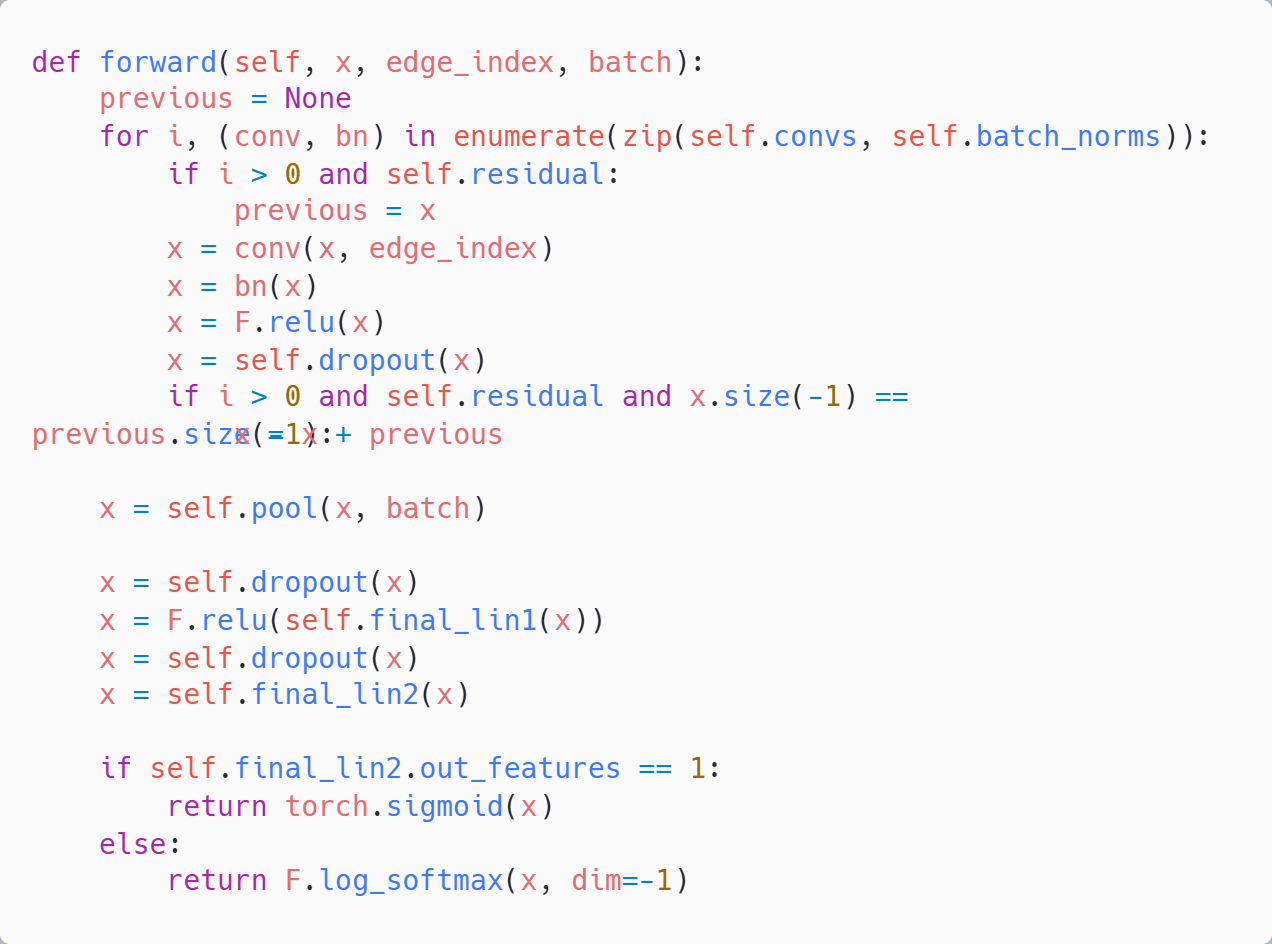
\includegraphics[width=1\textwidth]{images/forward propagation.png}  % Menyisipkan gambar dengan lebar setengah lebar teks
%     \caption{Kode forward propagation model GCN}  % Menambahkan keterangan gambar
%     \label{fig:forward propagation}  % Menambahkan label untuk referensi
% \end{figure}

Pemilihan arsitektur ini dilakukan karena model ini mampu mencegah penurunan kinerja yang kerap muncul pada jaringan graf melalui penerapan \textit{residual learning}, yakni \textit{skip-connection} yang menjaga aliran gradien dan mencegah \textit{oversmoothing} fitur node. Arsitektur ini mengekstraksi representasi tiap node melalui lapisan \textit{GCNConv}, menstabilkannya dengan \textit{Batch Normalization}, lalu merangkum seluruh node menjadi satu vektor graf memakai \textit{global pooling}. \textit{Skip-connection residual} dipakai untuk menahan gejala \textit{oversmoothing} saat lapisan bertambah banyak, sebelum representasi akhir diproses MLP \textit{head} untuk menghasilkan probabilitas prediksi. \par

\subsection{Pelatihan Model} \label{III.pelatihan}
Setelah arsitektur model dibangun, langkah berikutnya adalah pelatihan model. Pada tahap ini, model GCN akan dilatih menggunakan dataset yang sudah diproses dan telah dibagi menggunakan teknik 5-Fold seperti pada Subbab \ref{III.prapemrosesan}. Proses pelatihan akan melibatkan pembelajaran pola-pola posisi tubuh dan aktivitas lainnya pada lansi berdasarkan data \textit{pose landmark}. Model ini dilatih dengan menggunakan berbagai
\textit{hyperparameter} dengan nilai default seperti yang dapat dilihat pada Tabel \ref{table:3. hyperparamter default} serta menerapkan studi ablasi dengan rinciannya dapat dilihat pada Tabel \ref \par

% \textit{Optimizer} adalah algoritma yang digunakan untuk meminimalkan fungsi kerugian (\textit{loss function}) dengan tujuan mencari input yang menghasilkan output dengan nilai maksimum atau minimum pada suatu fungsi. \textit{Optimizer} memiliki peran dalam menentukan laju konvergensi dan stabilitas model menuju solusi yang optimal, serta mempengaruhi efisiensi proses pelatihan \cite{Lee2023}. Salah satu faktor yang mempengaruhi kinerja \textit{optimizer} adalah ukuran \textit{batch size}, yang merujuk pada jumlah sampel pelatihan yang diproses dalam satu iterasi saat data melewati jaringan \textit{neural}. Ukuran \textit{batch size} yang sering digunakan dalam banyak model Saat ini adalah 32 dan 64 \cite{Muralidhar2024}. \par

% Selain itu, \textit{learning rate} adalah parameter lain yang memainkan peran kunci dalam proses pelatihan, karena menentukan seberapa besar perubahan yang diterapkan pada bobot model setiap kali iterasi. Pemilihan \textit{learning rate} yang optimal sangat penting; jika \textit{learning rate} terlalu kecil, proses pelatihan bisa memakan waktu lebih lama untuk mencapai konvergensi. Sebaliknya, jika \textit{learning rate} terlalu besar, model bisa melewatkan titik minimum yang seharusnya dicapai, sehingga menyebabkan proses pembelajaran menjadi kurang efektif atau bahkan tidak stabil \cite{Xu2019}. Oleh karena itu, pemilihan \textit{learning rate} yang tepat sangat menentukan keberhasilan pelatihan model dan keberhasilan optimasi dalam mencapai solusi yang optimal. Pada penelitian ini digunakan \textit{learning rate} bawaan, yaitu 0,001 untuk \textit{optimizer} \textit{Adam}. \par

\subsection{Evaluasi Model} \label{III.evaluasi}
Setelah model dilatih, langkah selanjutnya adalah evaluasi performa model. Pada tahap ini, model diuji menggunakan data yang tidak digunakan dalam pelatihan yaitu 20\% data uji yang disediakan dalam setiap \textit{fold} untuk mengukur  \textit{accuracy}, \textit{precision}, \textit{recall}, dan \textit{F-1 Score}. Hasil evaluasi ini akan difokuskan pada metriks \textit{accuracy} untuk menentukan seberapa tepatnya model mampu mendeteksi posisi jatuh pada lansia. Pengukuran performa model secara keseluruhan, 5 nilai metriks  \textit{accuracy} dari hasil pelatihan masing-masing \textit{fold} akan dirata-ratakan sebagai nilai performa akhir. \par

\subsubsection{Percobaan Utama dengan Pengaturan Hyperparamter Default} \label{III.evaluasi default}
Subbab ini menyajikan nilai hyperpamater untuk percobaan utama agar menguji kemampuan model dalam mengklasifikasikan posisi jatuh dan tidak jatuh terhadap keseluruhan dataset. Pelatihan ini dilakukan menggunakan pengaturan hyperparameter \textit{default} yang dirumuskan dari praktik umum di literatur dan dokumentasi \textit{Pytorch}. Rincian nilai yang digunakan meliputi \textit{Optimizer}, \textit{Learning Rate}, \textit{Weight Decay}, \textit{Batch Size}, \textit{DropOut}, \textit{Epoch}, \textit{Hidden Channel}, serta \textit{Residual} dirangkum pada Tabel \ref{table:3. hyperparamter default} berikut sebagai acuan eksperimen utama sebelum eksplorasi lebih lanjut.

\begin{longtable}{| c | >{\raggedright\arraybackslash}p{0.23\textwidth} | >{\raggedright\arraybackslash}p{0.18\textwidth} | > {\raggedright\arraybackslash}p{0.38\textwidth} |}
    \caption{Nilai Default \textit{hyperparameter} model.}
    \label{table:3. hyperparamter default}
    \hline
    \centering \textbf{No} & \centering \textbf{Hyperparameter} & \centering \textbf{Nilai Default} & \centering \textbf{Keterangan}\hline
    \endfirsthead % Header di halaman pertama
    \hline
    \centering \textbf{No} & \centering \textbf{Hyperparameter} & \centering \textbf{Nilai Default} & \centering \textbf{Keterangan}
    \endhead % Header di halaman berikutnya
    \hline
    \endfoot
    \hline
    \endlastfoot
    1 & \textit{Optimizer} & AdamW & disarankan oleh H. Vo et al pada tahun 2024 dalam paper berjudul \textit{Exploring multiple optimization algorithms in transfer learning with EfficientNet models for agricultural insect classification} \cite{Vo2024} karena secara konsisten menunjukkan kinerja yang lebih unggul dibandingkan dengan algoritma \textit{optimizer} lain. \\ \hline
    2 & \textit{Learning Rate} & 1e-3 & Tidak ada nilai default dari dokumentasi Pytorch, sehingga nilai default diambil dari paper \textit{DeepGCNs: Making GCNs Go as Deep as CNNs} oleh G.Li et al pada tahun 2021 \cite{Li2021}\\ \hline
    3 & weight decay & 1e-5 & Tidak ada nilai default dari dokumentasi Pytorch, sehingga diambil nilai default dari paper \textit{Hybrid protein-ligand binding residue prediction with protein language models: Does the structure matter?} oleh H. Gamouh et al pada tahun 2025 \cite{Gamouh2025} \\ \hline
    4 & Batch Size & 32 & Tidak ada nilai default dari dokumentasi Pytorch, sehingga diambil nilai default dari paper \textit{Hybrid protein-ligand binding residue prediction with protein language models: Does the structure matter?} oleh H. Gamouh et al pada tahun 2025 \cite{Gamouh2025} \\ \hline
    5 & DropOut & 0.3 & Tidak ada nilai default dari dokumentasi Pytorch, sehingga nilai default diambil dari paper \textit{DeepGCNs: Making GCNs Go as Deep as CNNs} oleh G.Li et al pada tahun 2021 \cite{Li2021} \\ \hline
    6 & epoch & 100 & Tidak ada nilai default dari dokumentasi Pytorch, sehingga nilai default diambil dari paper \textit{DeepGCNs: Making GCNs Go as Deep as CNNs} oleh G.Li et al pada tahun 2021 \cite{Li2021} \\ \hline
    7 & Hidden Channel & [64, 32, 32, 32, 32] & Tidak ada nilai default dari dokumentasi Pytorch, sehingga nilai default diambil dari paper \textit{DeepGCNs: Making GCNs Go as Deep as CNNs} oleh G.Li et al pada tahun 2021 \cite{Li2021} \\ \hline 
    8 & Residual & True & Tidak ada nilai default dari dokumentasi Pytorch, sehingga nilai default diambil dari paper \textit{DeepGCNs: Making GCNs Go as Deep as CNNs} oleh G.Li et al pada tahun 2021 \cite{Li2021} karena menghasilkan stabilitas pelatihan yang konsisten di semua kedalaman layer \\ 
    \hline
\end{longtable}

Tabel \ref{table:3. hyperparamter default} merangkum pengaturan dasar yang digunakan pada percobaan utama sebagai titik awal yang konsisten untuk klasifikasi jatuh/tidak jatuh berbasis GCN. AdamW dipilih sebagai \textit{optimizer} karena stabil pada pembelajaran graf skala kecil-menengah dan cenderung memberikan generalisasi yang baik. \textit{Learning rate} 1e-3 dipakai sebagai nilai awal yang agresif namun masih stabil, sedangkan \textit{weight decay} 1e-5 ditetapkan untuk memberikan regularisasi ringan guna menekan \textit{overfitting} pada data \textit{skeleton pose}. Batch size 32 menyeimbangkan stabilitas estimasi gradien dan keterbatasan memori, sementara dropout 0{,}3 diterapkan pada lapisan representasi untuk mengendalikan kompleksitas model. Proses pelatihan dijalankan selama 100 epoch namun tetap menerapkan \textit{early stopping} untuk memberi kesempatan konvergensi tanpa overtraining, dengan konfigurasi \textit{hidden channel} [64, 32, 32, 32, 32] sebagai kompromi antara kapasitas representasi dan efisiensi komputasi. Selain itu, \textit{residual connection} diaktifkan (\textit{True}) guna memperlancar aliran gradien pada tumpukan lapisan GCN dan meningkatkan stabilitas pelatihan. Konfigurasi ini menjadi acuan baku bagi eksperimen dasar sebelum dilakukan penelusuran lebih lanjut pada subbab \ref{III.evaluasi ablasi}.

\subsubsection{Percobaan Tambahan Berdasarkan Studi Ablasi} \label{III.evaluasi ablasi}
Subbab ini memaparkan percobaan tambahan dalam bentuk studi ablasi untuk menilai kontribusi dan sensitivitas komponen-komponen kunci pada model GCN. Studi ablasi adalah prosedur eksperimen yang memvariasikan satu faktor pada satu waktu, sementara faktor lain ditahan pada konfigurasi \textit{default} guna mengisolasi pengaruh faktor tersebut terhadap kinerja model. Tujuan utamanya yaitu mengidentifikasi komponen yang paling berpengaruh terhadap performa, memahami trade-off antara akurasi, serta memperoleh konfigurasi yang lebih \textit{robust} terhadap variasi data. Pendekatan ini membantu menakar apakah perbaikan kinerja berasal dari penyesuaian tertentu (misalnya \textit{optimizer} atau \textit{learning rate}) atau sekadar efek samping dari kombinasi pengaturan yang tidak terkontrol.

Fokus ablasi pada subbab ini mencakup lima \textit{hyperparameter} inti yang paling berpotensi memengaruhi dinamika pembelajaran, yakni \textit{Optimizer}, \textit{Learning Rate}, \textit{Weight Decay}, \textit{Batch Size}, serta \textit{DropOut}. Setiap variasi diuji dengan menahan komponen lain pada pengaturan \textit{default} yang telah didefinisikan pada percobaan utama, dan dievaluasi menggunakan metrik akurasi, \textit{recall}, \textit{precision}, dan \textit{F1-score} agar hasilnya terbandingkan secara adil. Rincian cakupan nilai untuk tiap \textit{hyperparameter} yang akan diuji beserta skenario variasinya dirangkum pada Tabel \ref{table:3. ablasi hyperparamter} berikut sebagai acuan pelaksanaan dan pembacaan hasil studi ablasi.\par

\begin{longtable}{| c | >{\raggedright\arraybackslash}p{0.23\textwidth} | >{\raggedright\arraybackslash}p{0.18\textwidth} | > {\raggedright\arraybackslash}p{0.38\textwidth} |}
    \caption{Variasi nilai \textit{hyperparameter} model.}
    \label{table:3. ablasi hyperparamter}
    \hline
    \centering \textbf{No} & \centering \textbf{Hyperparameter} & \centering \textbf{Variasi} & \centering \textbf{Keterangan} \\ \hline
    \endfirsthead % Header di halaman pertama
    \hline
    \centering \textbf{No} & \centering \textbf{Hyperparameter} & \centering \textbf{Variasi} & \centering \textbf{Keterangan} \\ 
    \endhead % Header di halaman berikutnya
    \hline
    \endfoot
    \hline
    \endlastfoot
    1 & Optimizer & 1. AdamW \newline 2. RMSProp \newline 3. LION & Peneliti ingin membandingkan kinerja beberapa \textit{optimizer} dengan membatasi pada 3 \textit{optimizer} tersebut \\ \hline
    2 & Learning Rate & 1. 0.01 atau 1e-2 \newline 2. 0.001 atau 1e-3 \newline 3. 0.0001 atau 1e-4 & Penentuan variasi untuk melihat pengaruh kenaikan dan penurunan nilai hyperparameter terhadap akurasi pelatihan model \\ \hline
    3 & weight decay & 1. 1e-4 \newline 2. 1e-5 \newline 3. 1e-6 & Penentuan variasi untuk melihat pengaruh kenaikan dan penurunan nilai hyperparameter terhadap akurasi pelatihan model \\ \hline
    4 & Batch Size & 1. 16 \newline 2. 32 \newline 3. 64 & Penentuan variasi untuk melihat pengaruh kenaikan dan penurunan nilai hyperparameter terhadap akurasi pelatihan model \\ \hline
    5 & DropOut & 1. 0,2 \newline 2. 0,3 \newline 3. 0,4 & Penentuan variasi untuk melihat pengaruh kenaikan dan penurunan nilai hyperparameter terhadap akurasi pelatihan model \\ \hline
    - & Epoch & 100 & Hanya nilai default untuk pembatasan variasi \\ \hline
    - & Hidden Channel & [64, 32, 32, 32, 32] & Hanya nilai default untuk pembatasan variasi \\ \hline 
    - & Residual & True & Hanya nilai default untuk pembatasan variasi \\ 
    \hline
\end{longtable}

Tabel \ref{table:3. ablasi hyperparamter} merangkum ruang variasi yang digunakan pada studi ablasi ini, di mana setiap percobaan hanya memodifikasi satu \textit{hyperparameter} sementara yang lain dikunci pada konfigurasi \textit{default}. Variasi \textit{Optimizer} membandingkan AdamW, RMSProp, dan LION untuk menilai perbedaan dinamika gradien, stabilitas konvergensi, dan regularisasi implisit pada graf pose. \textit{Learning rate} divariasikan pada skala {1e-2, 1e-3, 1e-4} guna mengamati sensitivitas kecepatan belajar terhadap akurasi dan kestabilan pelatihan. \textit{Weight decay} diuji pada tiga nilai {1e-4, 1e-5, 1e-6} untuk melihat pengaruh regularisasi terhadap generalisasi. \textit{Batch size} {16, 32, 64} dipilih untuk mengevaluasi kompromi antara noise gradien, memori, dan throughput, sedangkan \textit{DropOut} {0,2; 0,3; 0,4} ditelaah sebagai kontrol kompleksitas representasi graf. Adapun epoch 100, hidden channel [64, 32, 32, 32, 32], dan residual \textit{True} tidak divariasikan dan dipertahankan tetap sebagai pembatas ruang pencarian agar perbandingan tidak terlalu luas. Seluruh variasi dievaluasi menggunakan metrik akurasi, dan \textit{loss} pada skema 1-fold, di mana pembagian 1-fold diambil dari fold yang memberikan pelatihan dengan akurasi terbaik pada percobaan utama. Hasil studi ablasi ini diharapkan menjadi dasar untuk mengidentifikasi konfigurasi paling berpengaruh dan kandidat pengaturan terbaik. \par

\section{Alat dan Bahan Tugas Akhir} \label{III.alat dan bahan}
Berbagai alat dan bahan yang akan digunakan dalam penelitian ini dijabarkan sebagai berikut. \par

\subsection{Alat} \label{III.alat}
\begin{enumerate}[noitemsep]
	\item Code editor Microsoft Visual Studio Code sebagai tempat pembuatan program model.
	\item Github untuk menampung dan melacak perkembangan hasil penelitian.
    \item Python versi 3.10 dengan pustaka utama PyTorch versi 2.9.0 dan Mediapipe untuk membangun program utama model.
    \item Jupyter Notebook untuk mempercepat eksperimen program hasil penelitian.
\end{enumerate}

\subsection{Bahan} \label{III.bahan}
Bahan sangat penting karena digunakan sebagai acuan pengembangan penelitian. Bahan yang akan digunakan dalam penelitian ini hanya berupa kumpulan video simulasi jatuh dan aktivitas sehari hari dalam lingkungan panti jompo. Penjelasan detail mengenai Datasetnya dapat dilihat pada Subbab \ref{III.pengumpulan data} \par

\section{Ilustrasi Metode Pengembangan/Pengukuran} \label{III.ilustrasi metode}
Pada subbab ini akan dijabarkan berbagai perhitungan penting dalam proses pengembangan dan pelatihan model. Berikut adalah contoh perhitungan pada lapisan konvolusi Graph Convolutional Network (GCN) untuk mempermudah pemahaman proses konvolusi menggunakan data dari 4 landmark, dengan masing-masing memiliki 3 fitur koordinat (x, y, z). Fitur-fitur ini digunakan untuk membentuk matriks $H^{(0)}$, yang akan menjadi input pertama dalam model. Matriks ini merepresentasikan posisi landmark manusia dalam koordinat tiga dimensi (x, y, z) untuk setiap landmark yang dianalisis. \par
\vspace{0.3cm}
\[
H^{(0)} = 
\begin{bmatrix}
0,5 & 0,5 & 0,5 \\
1,0 & 1,0 & 1,0 \\
1,5 & 1,5 & 1,5 \\
2,0 & 2,0 & 2,0
\end{bmatrix}
\]
\vspace{0.5cm}\par
Matriks adjacency menggambarkan hubungan antara landmark dalam graf. Misalnya, koneksi antar node (landmark) adalah sebagai berikut: node 1 terhubung dengan node 2 dan node 4; node 2 terhubung dengan node 1 dan node 3; node 3 terhubung dengan node 2 dan node 4; dan node 4 terhubung dengan node 1 dan node 3. Sementara itu, matriks derajat $D$ adalah matriks diagonal yang menunjukkan jumlah hubungan yang dimiliki oleh setiap node. Dalam kasus ini, node 1 terhubung dengan dua node lainnya (derajat = 2), node 2 terhubung dengan dua node lainnya (derajat = 2), node 3 terhubung dengan dua node lainnya (derajat = 2), dan node 4 terhubung dengan dua node lainnya (derajat = 2).\par
\vspace{0.3cm}
$$
A = 
\begin{bmatrix}
0 & 1 & 0 & 1 \\
1 & 0 & 1 & 0 \\
0 & 1 & 0 & 1 \\
1 & 0 & 1 & 0
\end{bmatrix}
,
D = 
\begin{bmatrix}
2 & 0 & 0 & 0 \\
0 & 2 & 0 & 0 \\
0 & 0 & 2 & 0 \\
0 & 0 & 0 & 2 \\
\end{bmatrix}
$$
\vspace{0.5cm}\par

Pada lapisan pertama, bobot $W^{(0)}$ dianggap sebagai matriks berukuran $3 \times 3$, yang setiap elemennya diinisialisasi dengan nilai acak. Matriks bobot ini digunakan untuk memproyeksikan fitur input dari matriks $H^{(0)}$ ke dalam ruang fitur yang lebih tinggi. Proses ini sangat penting dalam jaringan saraf, karena bobot yang teroptimasi dengan baik akan memungkinkan model untuk mengenali pola-pola penting dalam data dan memperbaiki prediksi seiring dengan bertambahnya jumlah iterasi. Bobot yang diinisialisasi secara acak ini akan dipelajari dan disesuaikan selama proses pelatihan untuk mencapai hasil yang optimal.\par
\vspace{0.3cm}
  $$
  W^{(0)} = \begin{bmatrix}
  0,1 & 0,2 & 0,3 \\
  0,4 & 0,5 & 0,6 \\
  0,7 & 0,8 & 0,9 \\
  \end{bmatrix}
  $$
\vspace{0.5cm}\par
Normalisasi Matriks Adjacency dan Derajat dilakukan untuk memastikan bahwa informasi yang diteruskan melalui jaringan dihitung dengan cara yang seimbang dan terkontrol. Matriks derajat ter-normalisasi $\hat{D}$ diperoleh dengan menambahkan matriks identitas $I$ ke dalam matriks derajat $D$. Penambahan matriks identitas ini bertujuan untuk mempertahankan informasi asal node, sehingga setiap node dapat mempertahankan kontribusinya dalam proses propagasi informasi. Sementara itu, matriks adjacency ter-normalisasi $\hat{A}$ dibentuk dengan menambahkan matriks identitas $I$ ke dalam matriks adjacency $A$, yang mencerminkan hubungan antar node. Langkah ini sangat penting agar setiap node dapat memperhitungkan keterhubungannya dengan node lainnya, sekaligus mempertimbangkan pengaruh dari dirinya sendiri selama propagasi informasi dalam jaringan. \par
\vspace{0.3cm}
   $$
   \hat{D} = D + I = \begin{bmatrix}
   3 & 0 & 0 & 0 \\
   0 & 3 & 0 & 0 \\
   0 & 0 & 3 & 0 \\
   0 & 0 & 0 & 3 \\
   \end{bmatrix}
   ,
   \hat{A} = A + I = \begin{bmatrix}
   1 & 1 & 0 & 1 \\
   1 & 1 & 1 & 0 \\
   0 & 1 & 1 & 1 \\
   1 & 0 & 1 & 1 \\
   \end{bmatrix}
   $$
\vspace{0.5cm}\par
Setelah normalisasi matriks adjacency dan derajat dilakukan, langkah berikutnya dalam proses propagasi fitur adalah perhitungan normalisasi lebih lanjut. Matriks normalisasi ini merupakan invers dari akar kuadrat matriks derajat yang telah dinormalisasi. Proses ini bertujuan untuk mengatur bobot hubungan antar node dalam graf, sehingga informasi yang dipropagasikan antar node tidak terdistorsi oleh ketidakseimbangan jumlah koneksi setiap node. Dengan normalisasi ini, setiap node dapat memberikan kontribusi yang proporsional terhadap hasil akhir, berdasarkan hubungannya dengan node lainnya. Langkah ini sangat penting untuk memastikan bahwa kontribusi informasi dari masing-masing node dihitung secara adil selama proses propagasi.\par
\vspace{0.3cm}
   $$
   \hat{D}^{-1/2} = \begin{bmatrix}
   0,577 & 0 & 0 & 0 \\
   0 & 0,577 & 0 & 0 \\
   0 & 0 & 0,577 & 0 \\
   0 & 0 & 0 & 0,577 \\
   \end{bmatrix}
   $$
\vspace{0.5cm}\par
Setelah langkah normalisasi selesai, proses selanjutnya adalah propagasi informasi melalui jaringan. Pada tahap ini, informasi dari matriks fitur $H^{(0)}$ dipropagasikan dengan menggunakan rumus \ref{eq:propagasi} berikut.\par
\vspace{0.2cm}
\begin{align*}
    H^{(1)} = \sigma \left( \hat{D}^{- \frac{1}{2}} \hat{A} \hat{D}^{- \frac{1}{2}} H^{(0)} W^{(0)} \right)\\
\end{align*}

Di sini, matriks $H^{(0)}$, yang berisi fitur input pada lapisan pertama, digabungkan dengan matriks ter-normalisasi $\hat{D}^{-1/2}$ dan matriks adjacency $\hat{A}$. Pengalihan ini bertujuan untuk memperhitungkan hubungan antar node dalam graf dengan cara yang proporsional dan terkontrol. Selanjutnya, bobot $W^{(0)}$ diterapkan pada hasil penggabungan tersebut untuk memproyeksikan fitur ke ruang yang lebih tinggi. Proses ini memungkinkan informasi yang ada pada node-node dalam graf untuk dipertukarkan, disesuaikan, dan diperbarui berdasarkan keterhubungan mereka, menghasilkan representasi yang lebih kompleks dan bermakna pada lapisan berikutnya.

Setelah propagasi selesai, hasil output dari proses ini adalah matriks $H^{(1)}$, yang berisi fitur yang telah diperbarui dan dipropagasi ke seluruh node. Matriks output ini, yang berukuran $4 \times 3$, menunjukkan fitur hasil propagasi untuk masing-masing node pada lapisan pertama, dengan nilai-nilai yang telah diperbarui sesuai dengan hubungan antar node dan bobot yang dipelajari. Matriks ini menggambarkan bagaimana informasi dari node-node dalam graf saling mempengaruhi satu sama lain dan diperbarui sesuai dengan struktur graf yang ada. Sebagai contoh, hasilnya adalah sebagai berikut.\par
\vspace{0.3cm}
$$
H^{(1)} = 
\begin{bmatrix}
1,4 & 1,75 & 2,1 \\
1,2 & 1,5 & 1,8 \\
1,8 & 2,25 & 2,7 \\
1,6 & 2,0 & 2,4
\end{bmatrix}
$$
\vspace{0.5cm}\par

Selain perhitungan pada lapisan Graph Convolutional Network (GCN), terdapat juga perhitungan dalam rangkaian pelatihan model yang bertujuan untuk mengevaluasi kinerja model dalam mendeteksi posisi jatuh dan tidak jatuh pada lansia. Evaluasi kinerja dilakukan dengan mengukur akurasi deteksi terhadap dua kategori utama, yaitu posisi jatuh dan tidak jatuh. Tujuan dari evaluasi ini adalah untuk memastikan bahwa model dapat secara efektif membedakan antara kejadian jatuh dan aktivitas normal, sehingga dapat diandalkan dalam aplikasi pemantauan kesehatan lansia.\par

Prosedur evaluasi dimulai dengan pelatihan lima model GCN, di mana setiap model dilatih menggunakan data dari satu fold dalam skema 5-fold cross-validation. Selanjutnya, setiap model dievaluasi menggunakan data validation yang sudah disediakan dalam masing-masing fold untuk mengukur kinerjanya. Metrik evaluasi yang digunakan mencakup akurasi, presisi, recall, dan F1-score, yang dihitung berdasarkan hasil prediksi dan label sebenarnya dari data validation masing-masing fold. Setelah evaluasi, hasil dari kelima model tersebut dirata-rata untuk mendapatkan nilai kinerja keseluruhan. Terakhir, kinerja model GCN yang dikembangkan dibandingkan dengan metode deteksi jatuh lainnya yang ada dalam literatur untuk menilai keunggulan dan potensi perbaikan yang dapat dicapai melalui pendekatan berbasis GCN. \par
\vspace{10pt}

\begin{table}[h!]
\centering
\begin{tabular}{|c|c|c|}
\hline
\multirow{2}{*}{\textbf{Label Sebenarnya}} & \multicolumn{2}{c|}{\textbf{Label Prediksi}} \\
\cline{2-3} 
 & 1 (Positive) & 0 (Negative) \\
\hline
1 (Positive) & 50 & 5 \\
\hline
0 (Negative) & 10 & 200 \\
\hline
\end{tabular}
\caption{contoh nilai \textit{Confussion Matrix}}
\label{table:3.contoh confusion matrix}
\end{table}

Penilaian kinerja model menggunakan metrik evaluasi pada Gambar \ref{fig:confusion matrix}, dapat diilustrasikan seperti pada Tabel \ref{table:3.contoh confusion matrix} di mana hasil evaluasi untuk model pertama deteksi posisi jatuh pada lansia menunjukkan distribusi prediksi sebagai berikut.
\begin{enumerate}
    \item 50 True Positives (TP), yaitu terdapat 50 kasus jatuh yang benar-benar terdeteksi sebagai jatuh.
    \item 10 False Positives (FP), artinya ada 10 kasus tidak jatuh yang salah terdeteksi sebagai jatuh.
    \item 5 False Negatives (FN), berarti terdapat 5 kasus jatuh yang salah terdeteksi sebagai tidak jatuh.
    \item 200 True Negatives (TN), maksudnya ada 200 kasus tidak jatuh yang benar-benar terdeteksi sebagai tidak jatuh.
\end{enumerate}

berdasarkan data tersebut, perhitungan evaluasi lanjutan dapat dilakukan sebagai berikut.

\begin{enumerate}
    \item \textit{Accuracy}
    \vspace{20pt} 
    \begin{align*}
        \text{Accuracy} &= \frac{TP + TN}{TP + TN + FP + FN} \\
        &= \frac{50 + 200}{50 + 200 + 10 + 5} = \frac{250}{265} = 0.8571 \quad \text{atau} \quad 85.71\%
    \end{align*}
    
    \item \textit{Precision}
    \vspace{20pt} 
    \begin{align*}
        \text{Precision} &= \frac{TP}{TP + FP} \\
        &= \frac{50}{50 + 10} = 0,8333 \text{ atau}\ 83,3\%
    \end{align*}
    
    \item \textit{Recall}
    \vspace{20pt} 
    \begin{align*} 
        \text{Recall} &= \frac{TP}{TP + FN} \\ 
        &= \frac{50}{50 + 5} \times 100\% = 0,9091 \text{ atau}\ 90,91\%
    \end{align*}
    
    
    \item \textit{F1-Score}
    \vspace{20pt}
    \begin{align*}
        F1 &= 2 \times \frac{\text{Precision} \times \text{Recall}}{\text{Precision} + \text{Recall}} \\ 
        &= 2 \times \frac{0,8333 \times 0,9091}{0,8333 + 0,9091} = 0,8696 \text{ atau}\ 86,96\% 
    \end{align*}
\end{enumerate} 

\vspace{10pt}

Hasil perhitungan confusion matrix menunjukkan bahwa model berhasil mengidentifikasi 50 kasus jatuh dengan benar (True Positives), sementara 10 kasus tidak jatuh salah terdeteksi sebagai jatuh (False Positives). Selain itu, terdapat 5 kasus jatuh yang tidak terdeteksi (False Negatives), dan 200 kasus tidak jatuh yang terklasifikasi dengan benar sebagai tidak jatuh (True Negatives). Berdasarkan perhitungan ini, akurasi model adalah 85,71\%, yang menunjukkan bahwa model dapat mengklasifikasikan 85,71\% dari seluruh data dengan benar. Presisi sebesar 83,33\% mengindikasikan bahwa 83,33\% dari semua prediksi jatuh yang dilakukan oleh model memang benar-benar jatuh, sedangkan recall sebesar 90,91\% menunjukkan bahwa model berhasil mendeteksi 90,91\% dari seluruh kejadian jatuh yang sebenarnya. F1-score yang dihitung sebesar 86,96\% mencerminkan keseimbangan antara presisi dan recall, menunjukkan kinerja yang baik dalam mendeteksi jatuh dengan mempertimbangkan kedua metrik tersebut.
